\documentclass[11pt]{article}

\usepackage[a4paper,margin=1in]{geometry}
\usepackage{graphicx}
\usepackage{booktabs}
\usepackage{array}
\usepackage{longtable}
\usepackage{float}
\usepackage{caption}
\usepackage{subcaption}
\usepackage{hyperref}

\graphicspath{{epsilon_fmm/}{mac/}{theta_cr/}{timestep/}}

\title{Parameter Study}
\author{}
\date{}

\begin{document}

\maketitle

\section*{Test summary}

\begin{table}[H]
\centering
\caption{Summary of self-gravity solver parameter values in the study. Each row lists the parameter, its baseline value (used in the reference run), and the test values explored to assess sensitivity.}
\label{tab:solver_parameters}
\begin{tabular}{lcccc}
\hline
\textbf{Parameter} & \textbf{Baseline} & \multicolumn{3}{c}{\textbf{Test values}} \\
\hline
$\eta$ (timestep) & 0.002 & 0.0002 & 0.02 & — \\
MAC & geometric & adaptive & — & — \\
$\theta_{\mathrm{cr}}$ (geometric only) & 0.7 & 0.5 & — & — \\
$\epsilon_{\mathrm{fmm}}$ (FMM tolerance) & 0.001 & 0.0001 & 0.01 & 0.1 \\
\hline
\end{tabular}
\end{table}

\clearpage
\section*{$\epsilon_{\mathrm{fmm}}$}

\begin{figure}[H]
    \centering
    \begin{minipage}{\textwidth}
        \centering
        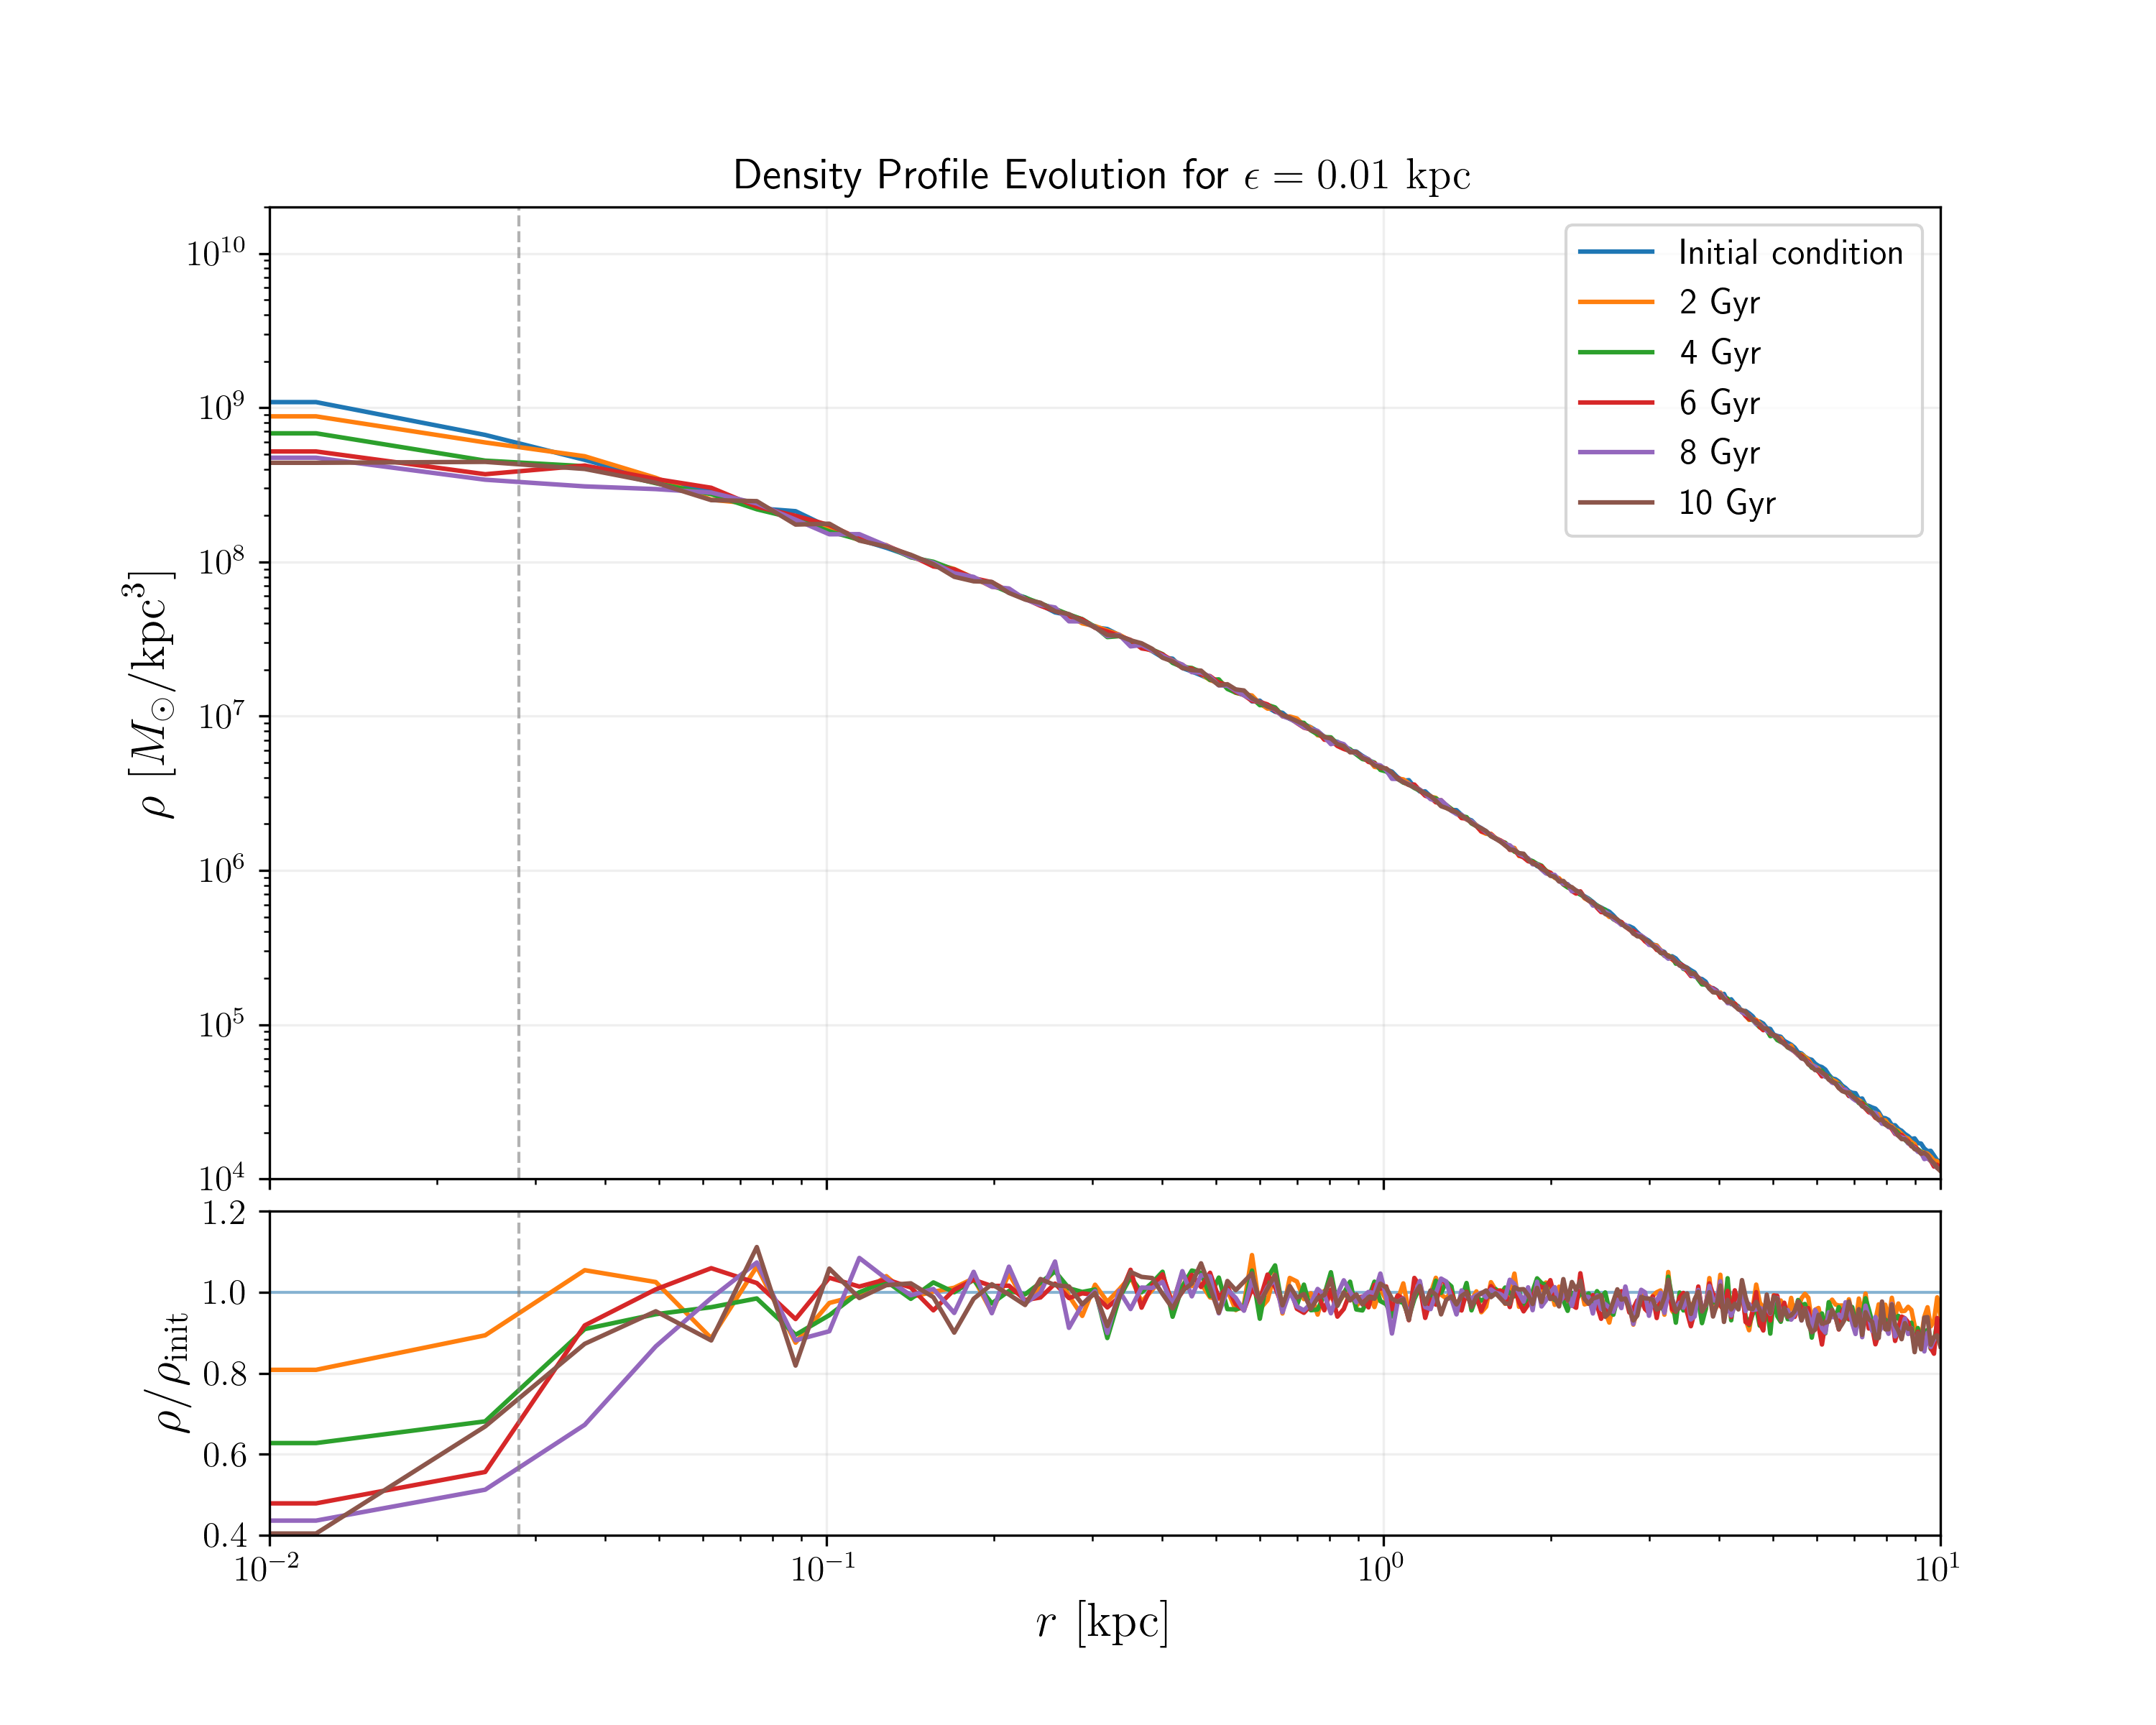
\includegraphics[width=0.48\textwidth]{density_evo_eps01_10.png}
        \hfill
        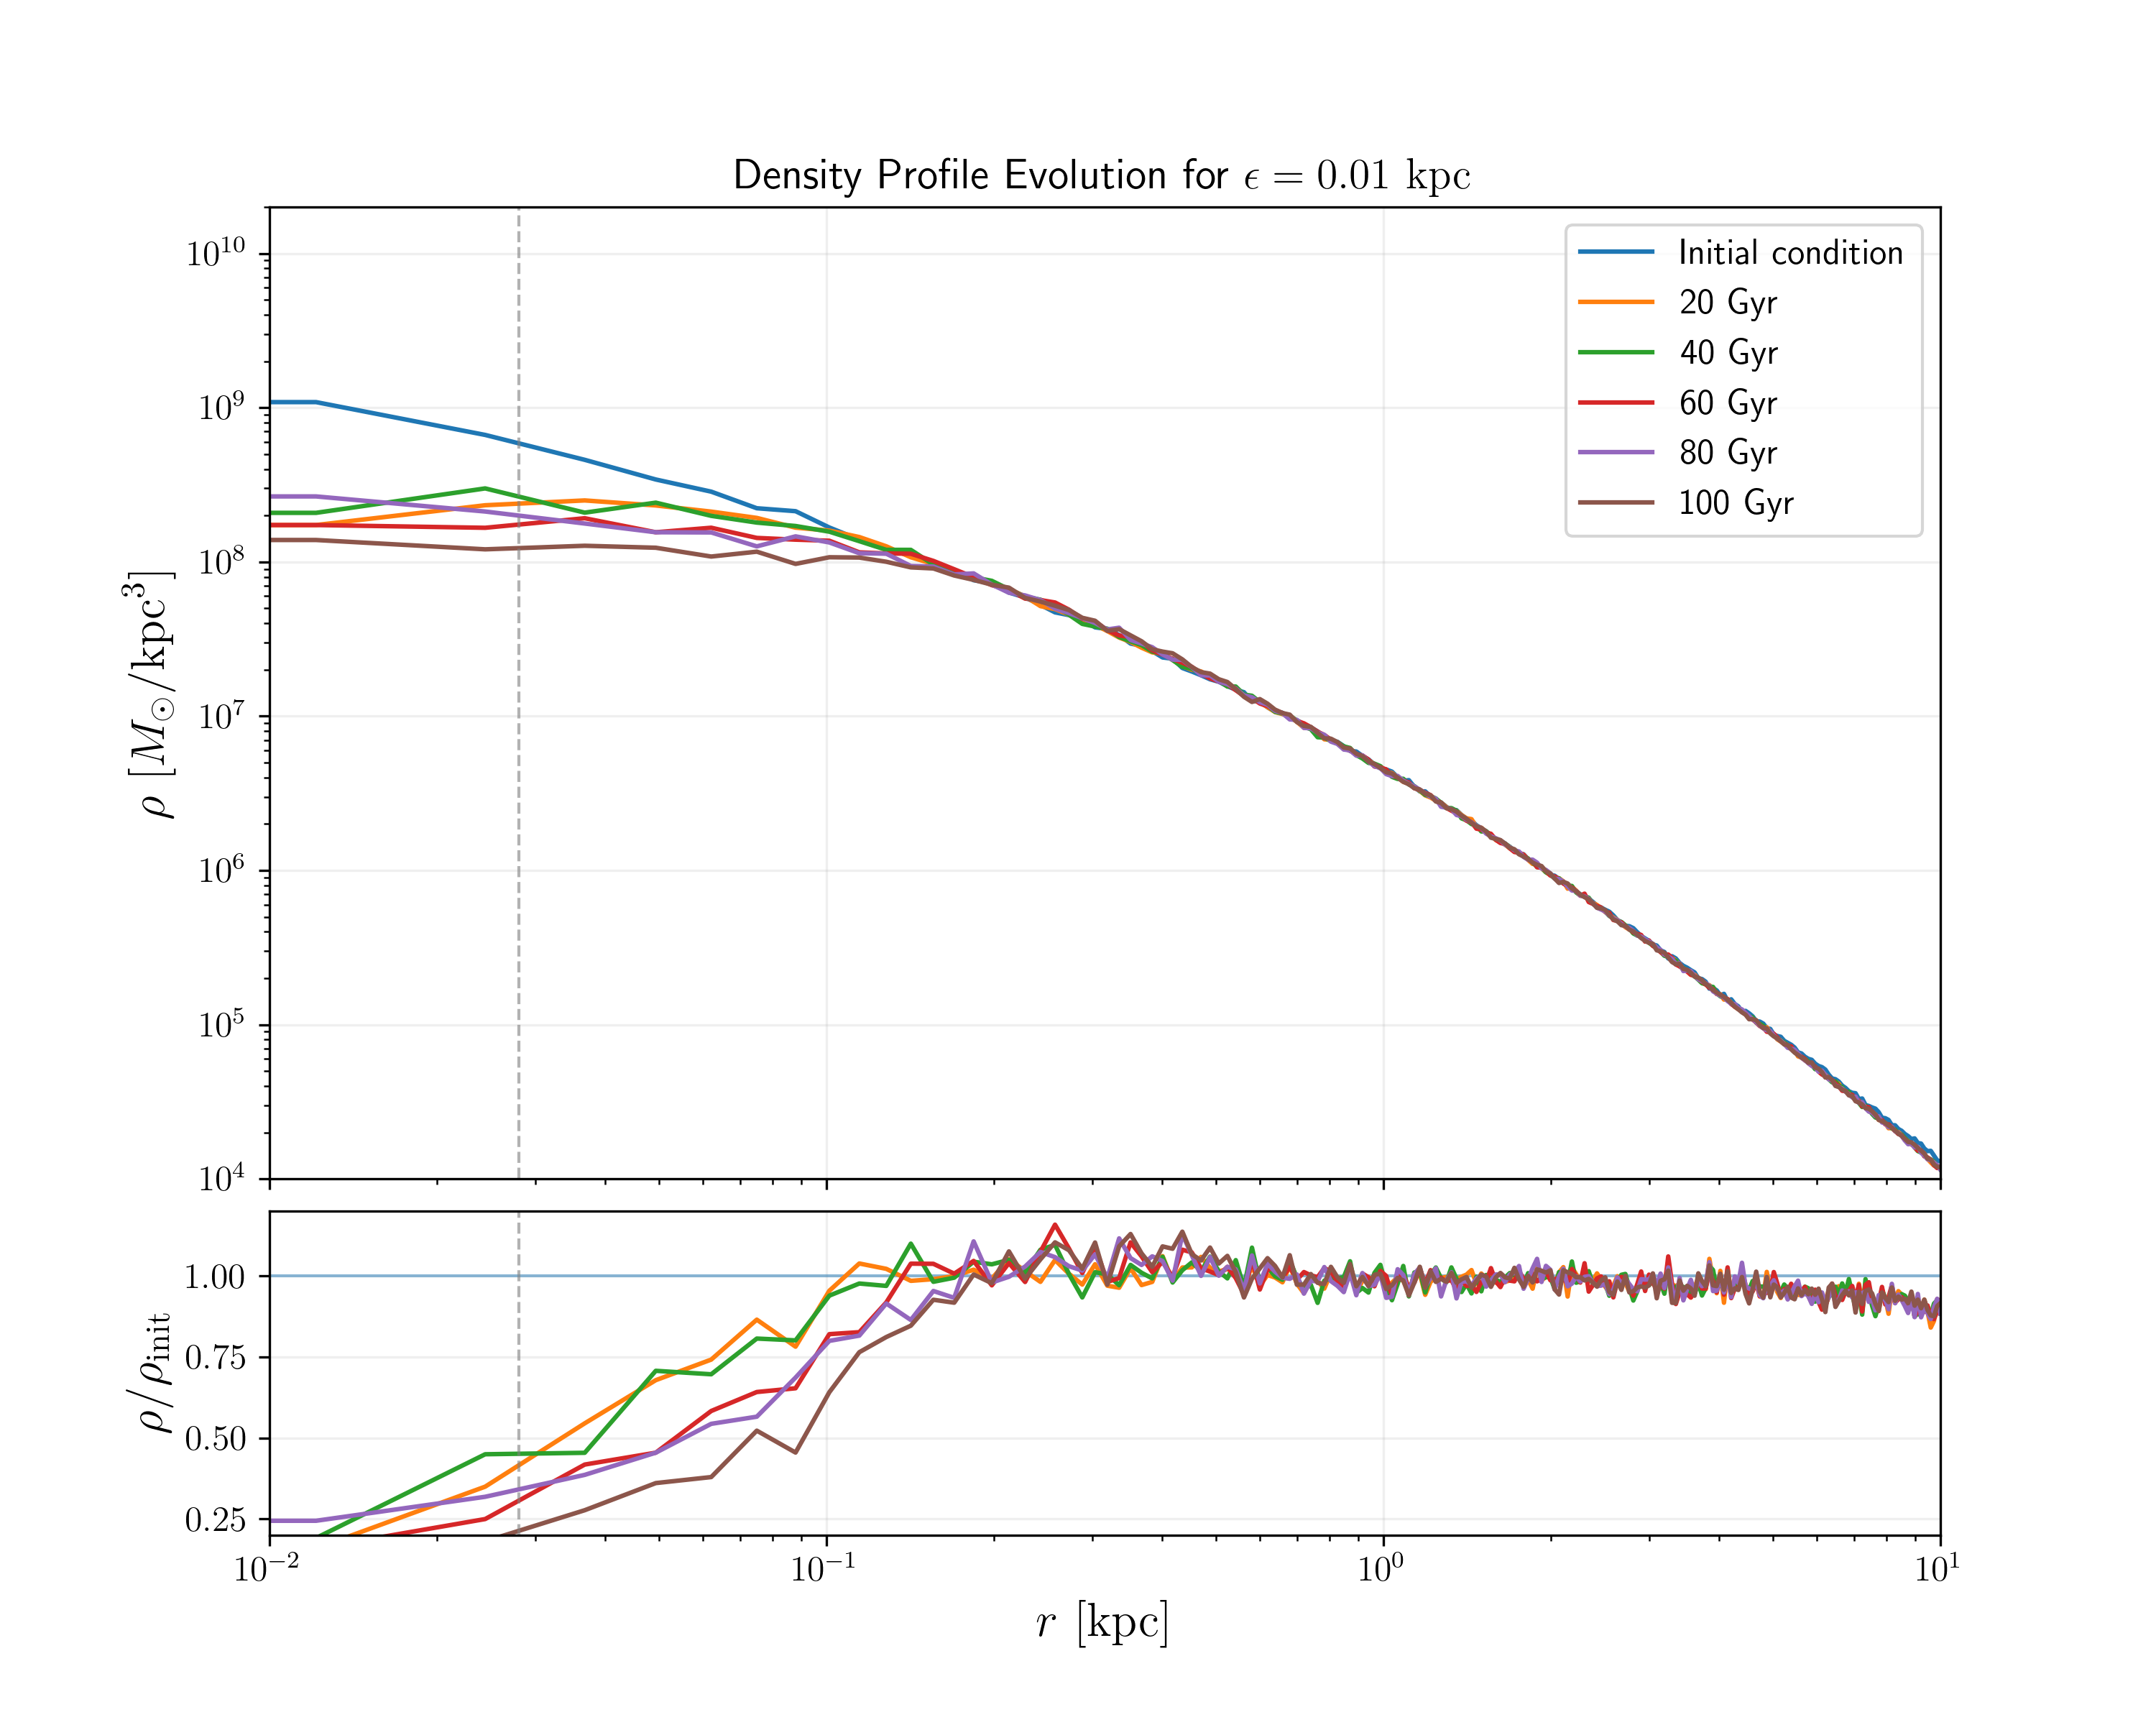
\includegraphics[width=0.48\textwidth]{density_evo_eps01_100.png}
        \\[0.5em]
        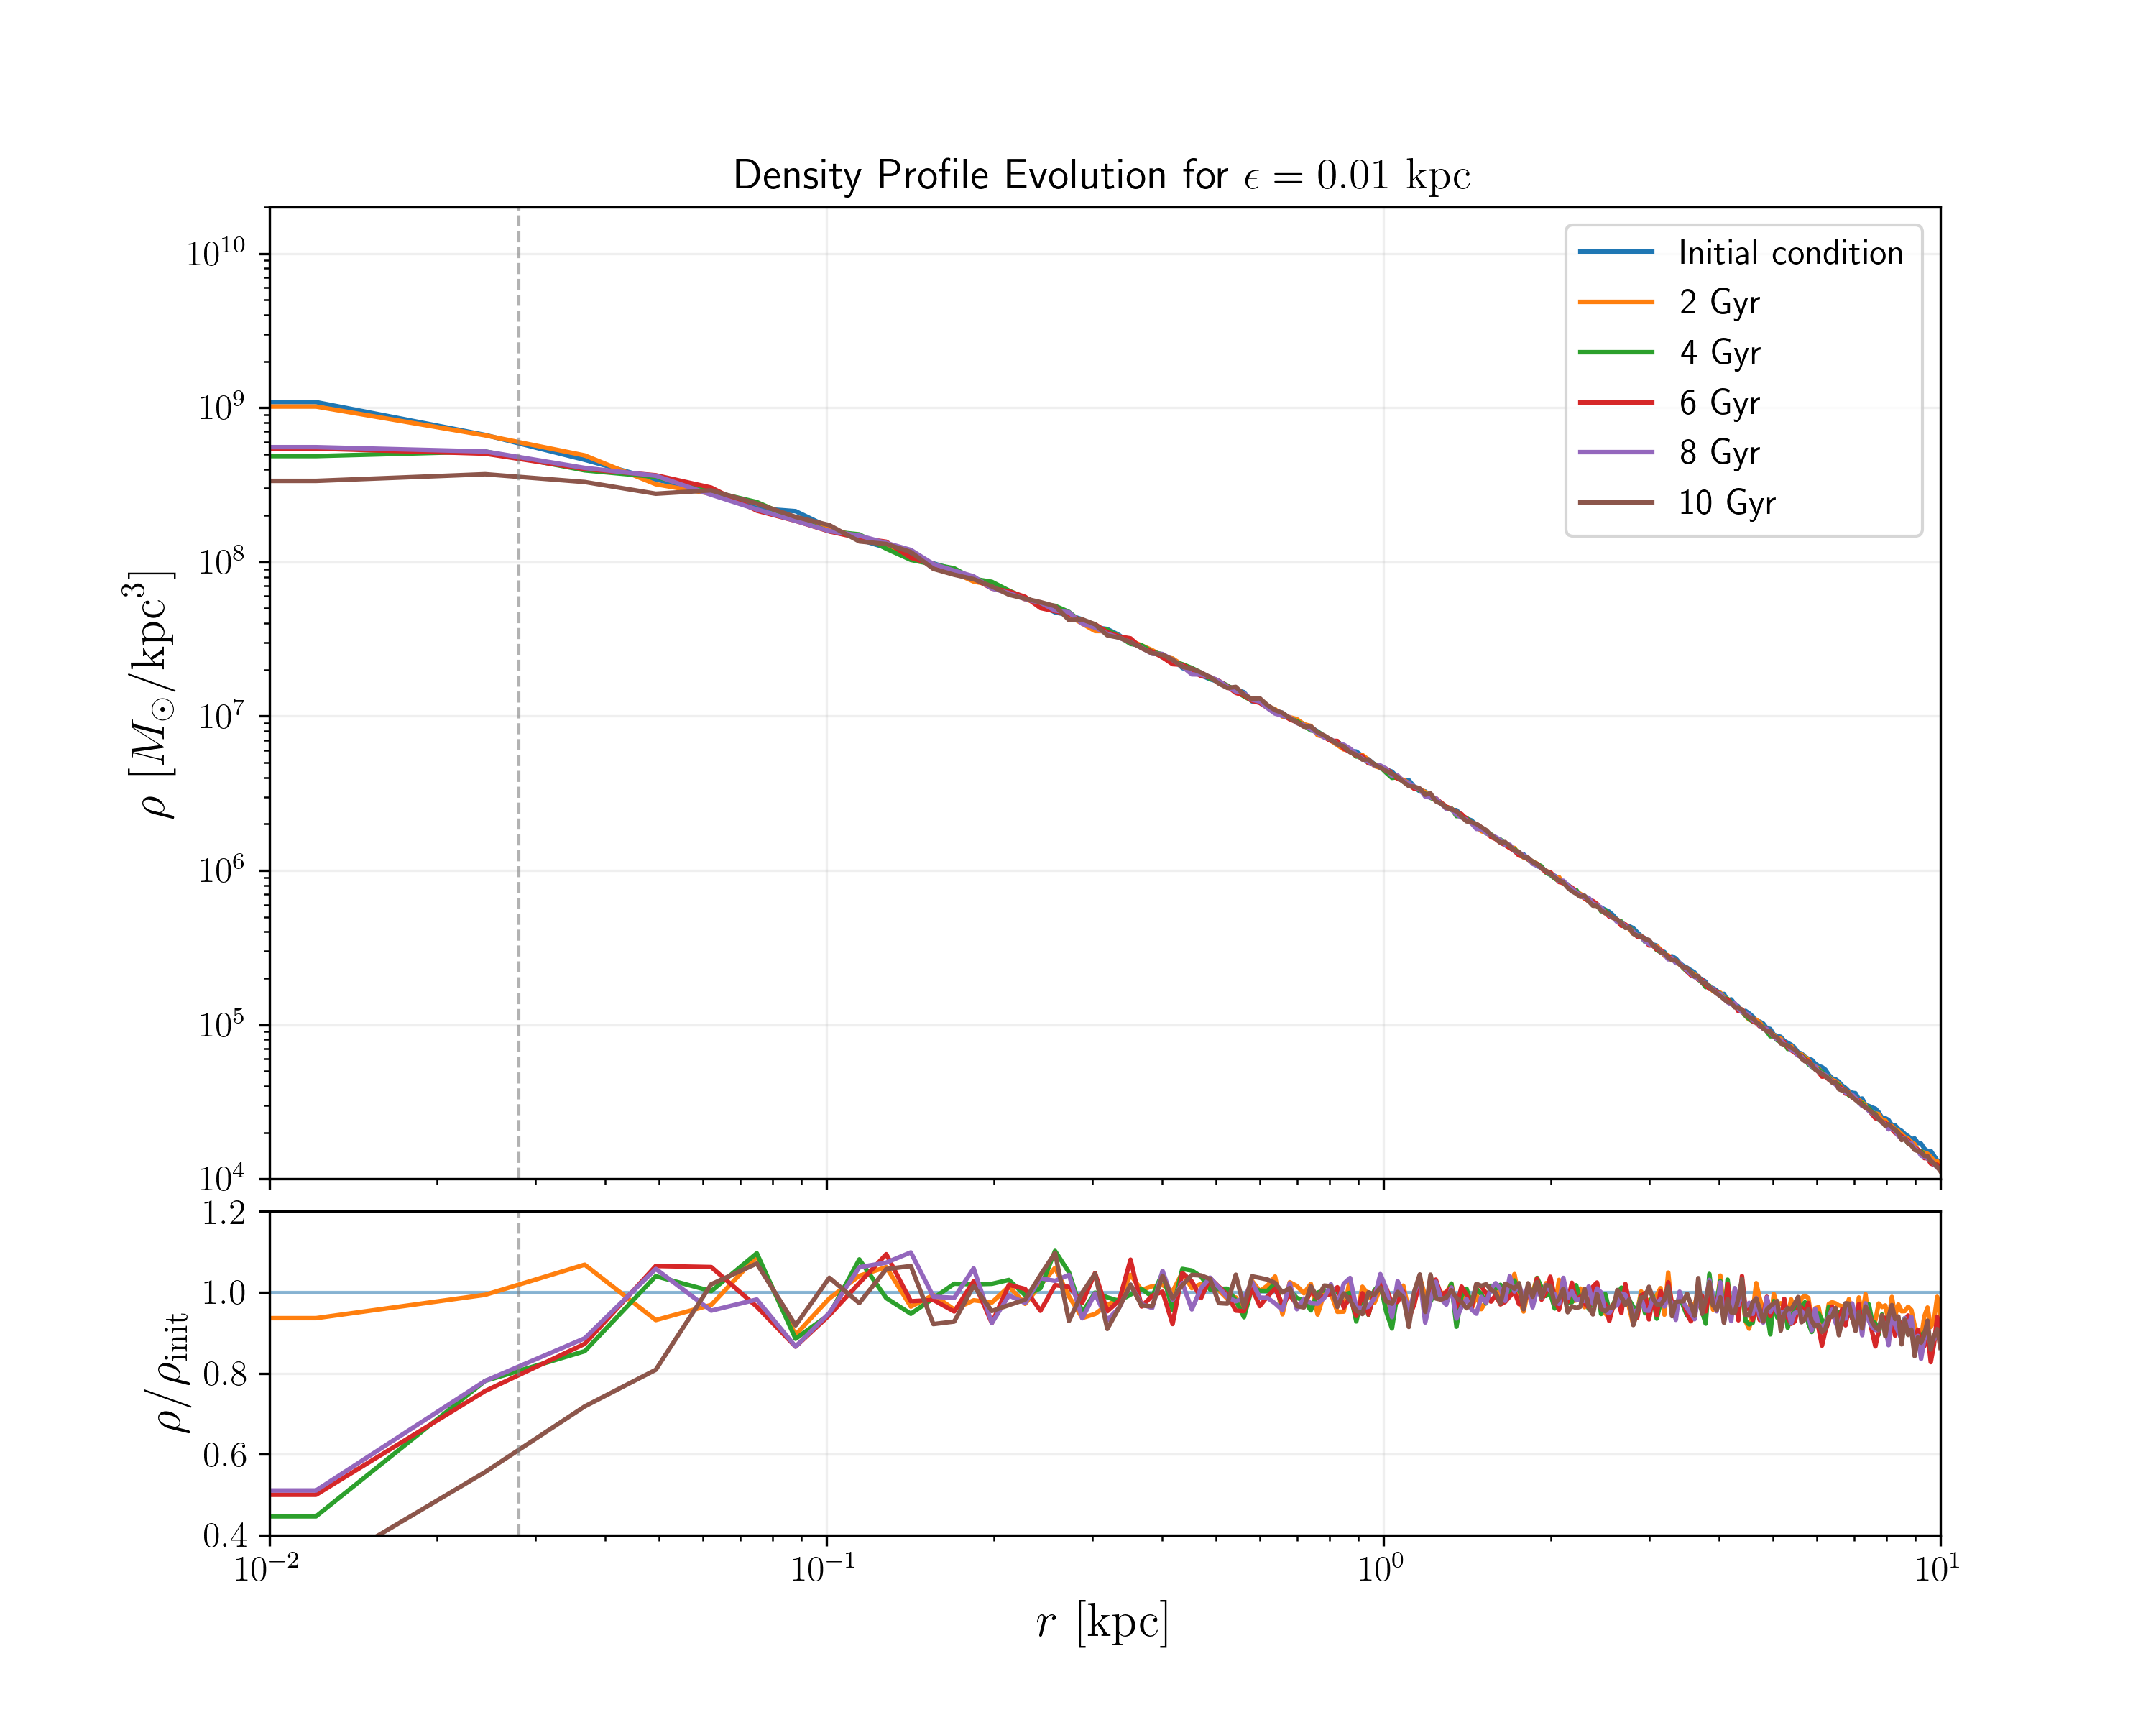
\includegraphics[width=0.48\textwidth]{density_evo_eps02_10.png}
        \hfill
        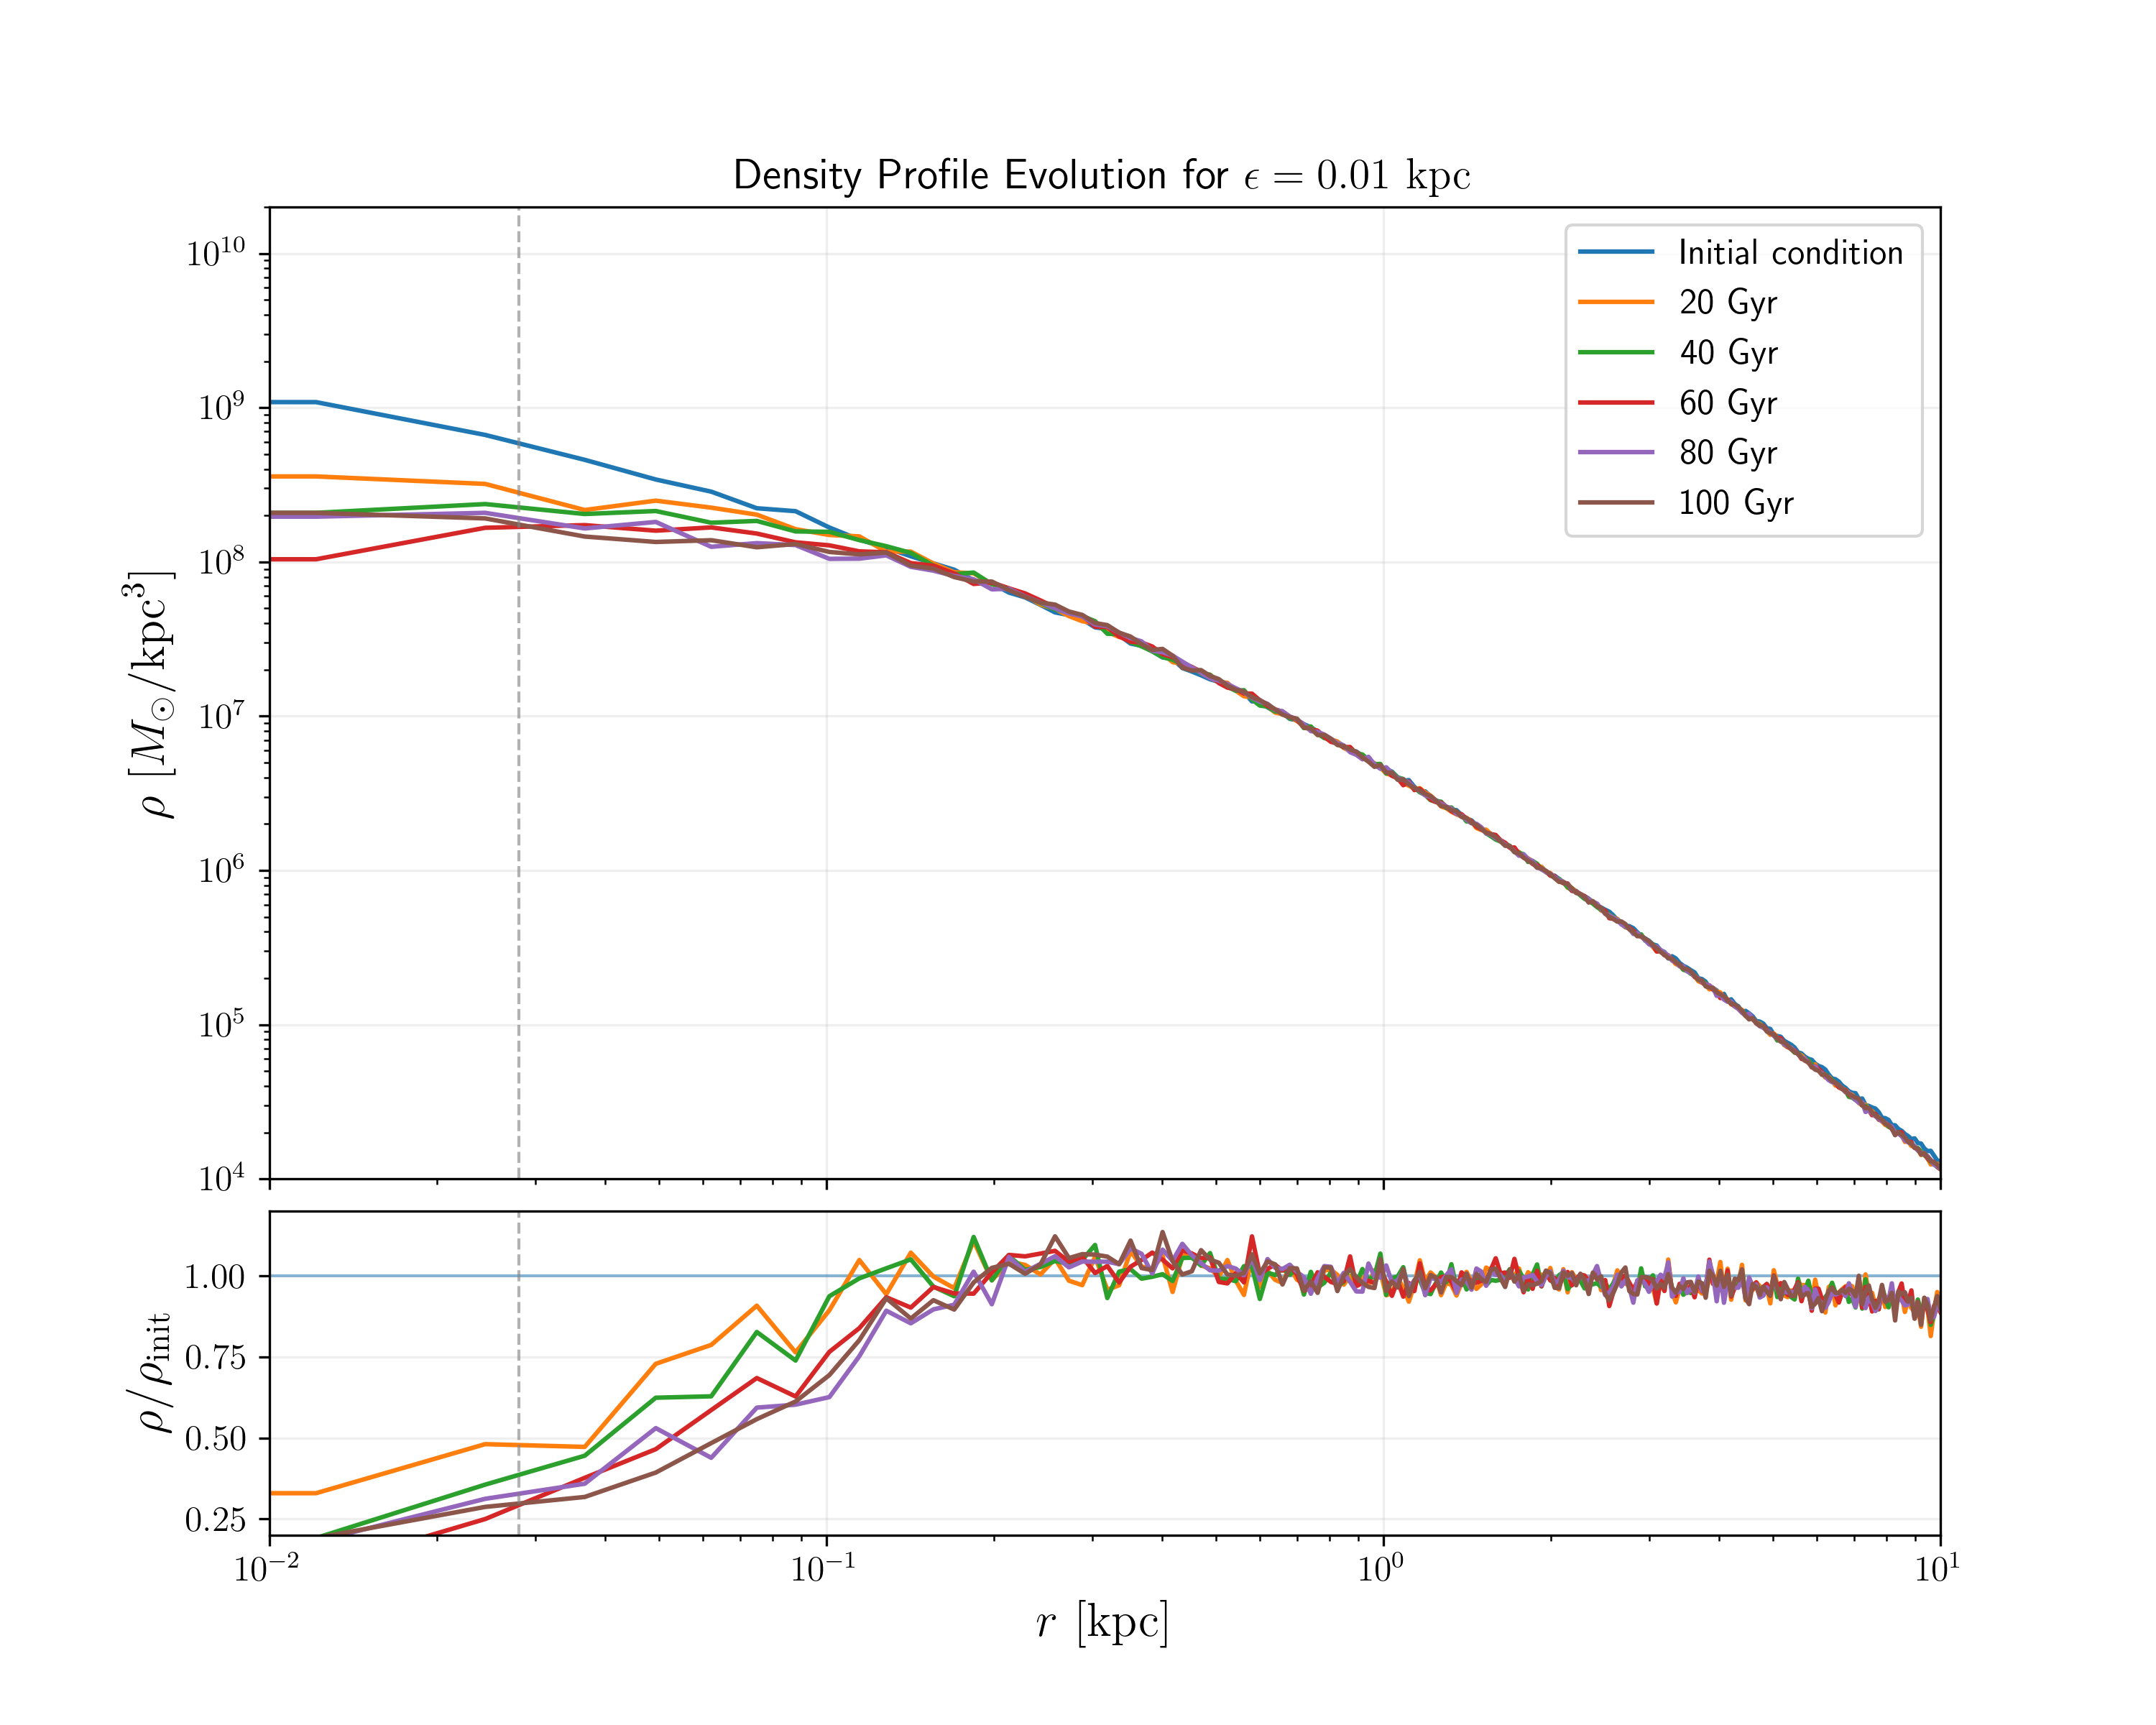
\includegraphics[width=0.48\textwidth]{density_evo_eps02_100.png}
        \\[0.5em]
        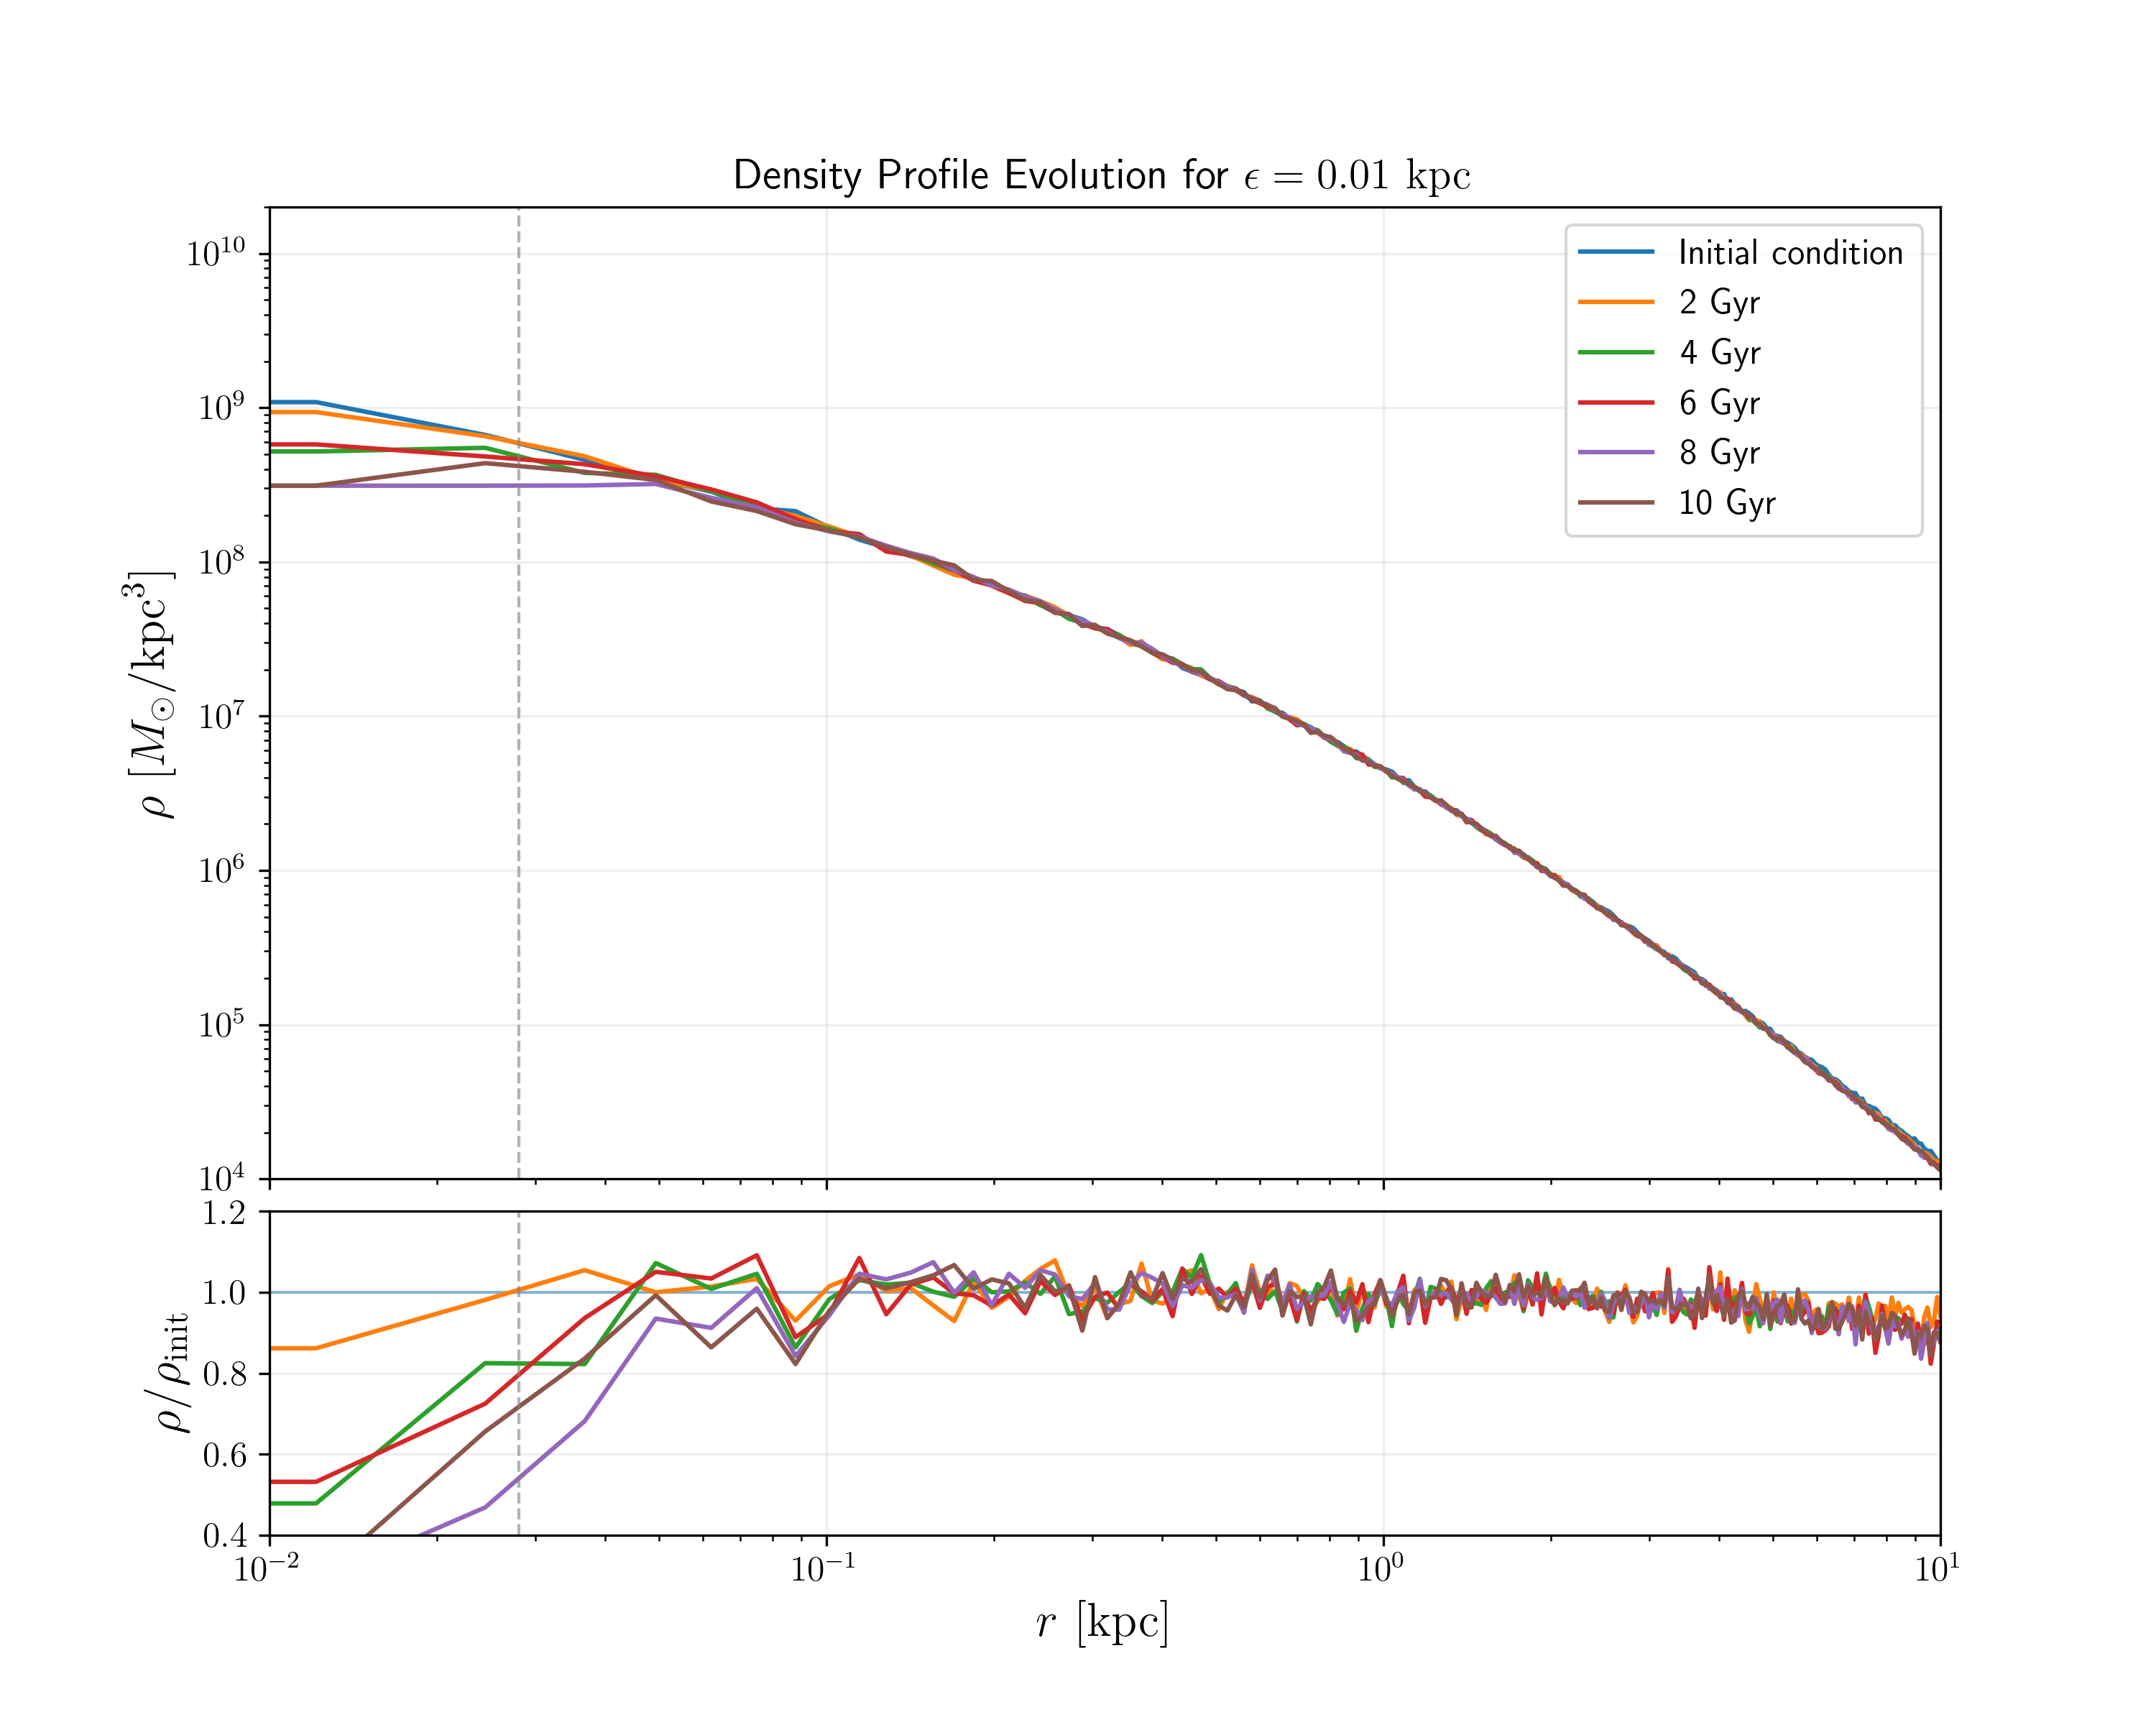
\includegraphics[width=0.48\textwidth]{density_evo_eps03_10.png}
        \hfill
        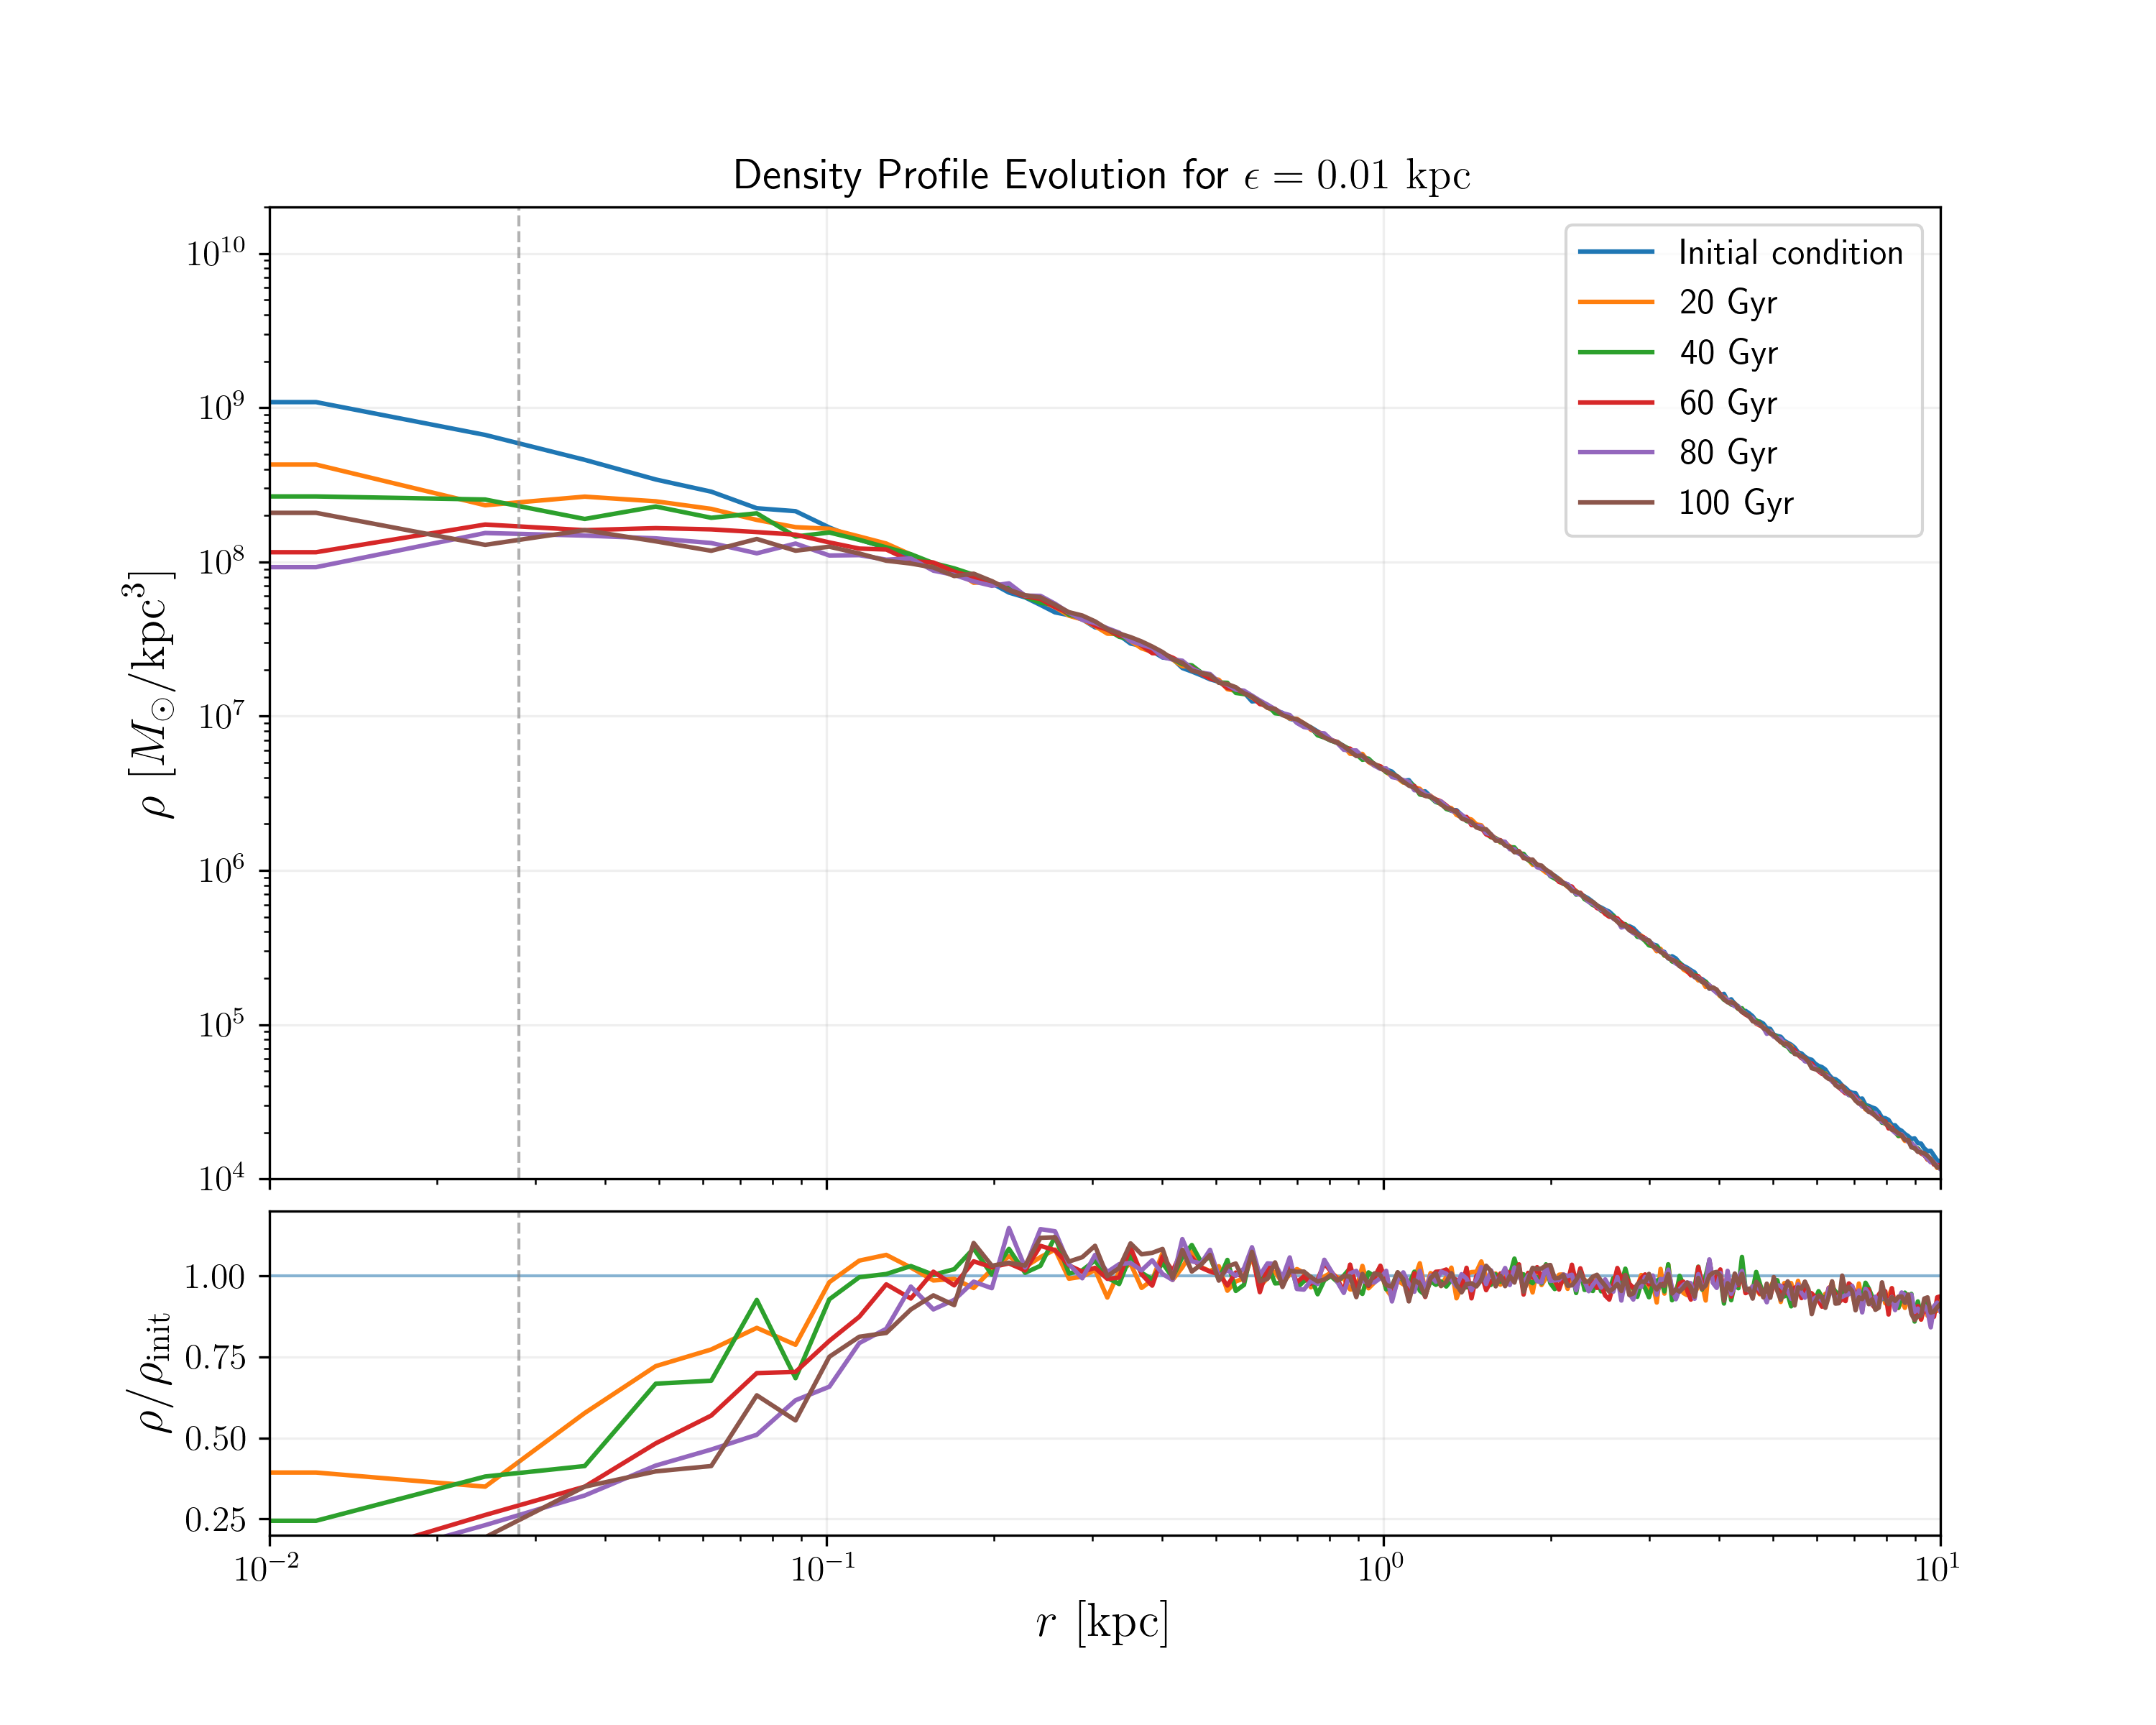
\includegraphics[width=0.48\textwidth]{density_evo_eps03_100.png}
    \end{minipage}
    \caption{Density evolution for $\epsilon_{\mathrm{fmm}}$ tests. Left-to-right, top-to-bottom: $\epsilon_{\mathrm{fmm}} = 0.01$ (step 10), $0.01$ (step 100), $0.0001$ (step 10), $0.0001$ (step 100), $0.1$ (step 10), $0.1$ (step 100).}
\end{figure}

\begin{figure}[H]
    \centering
    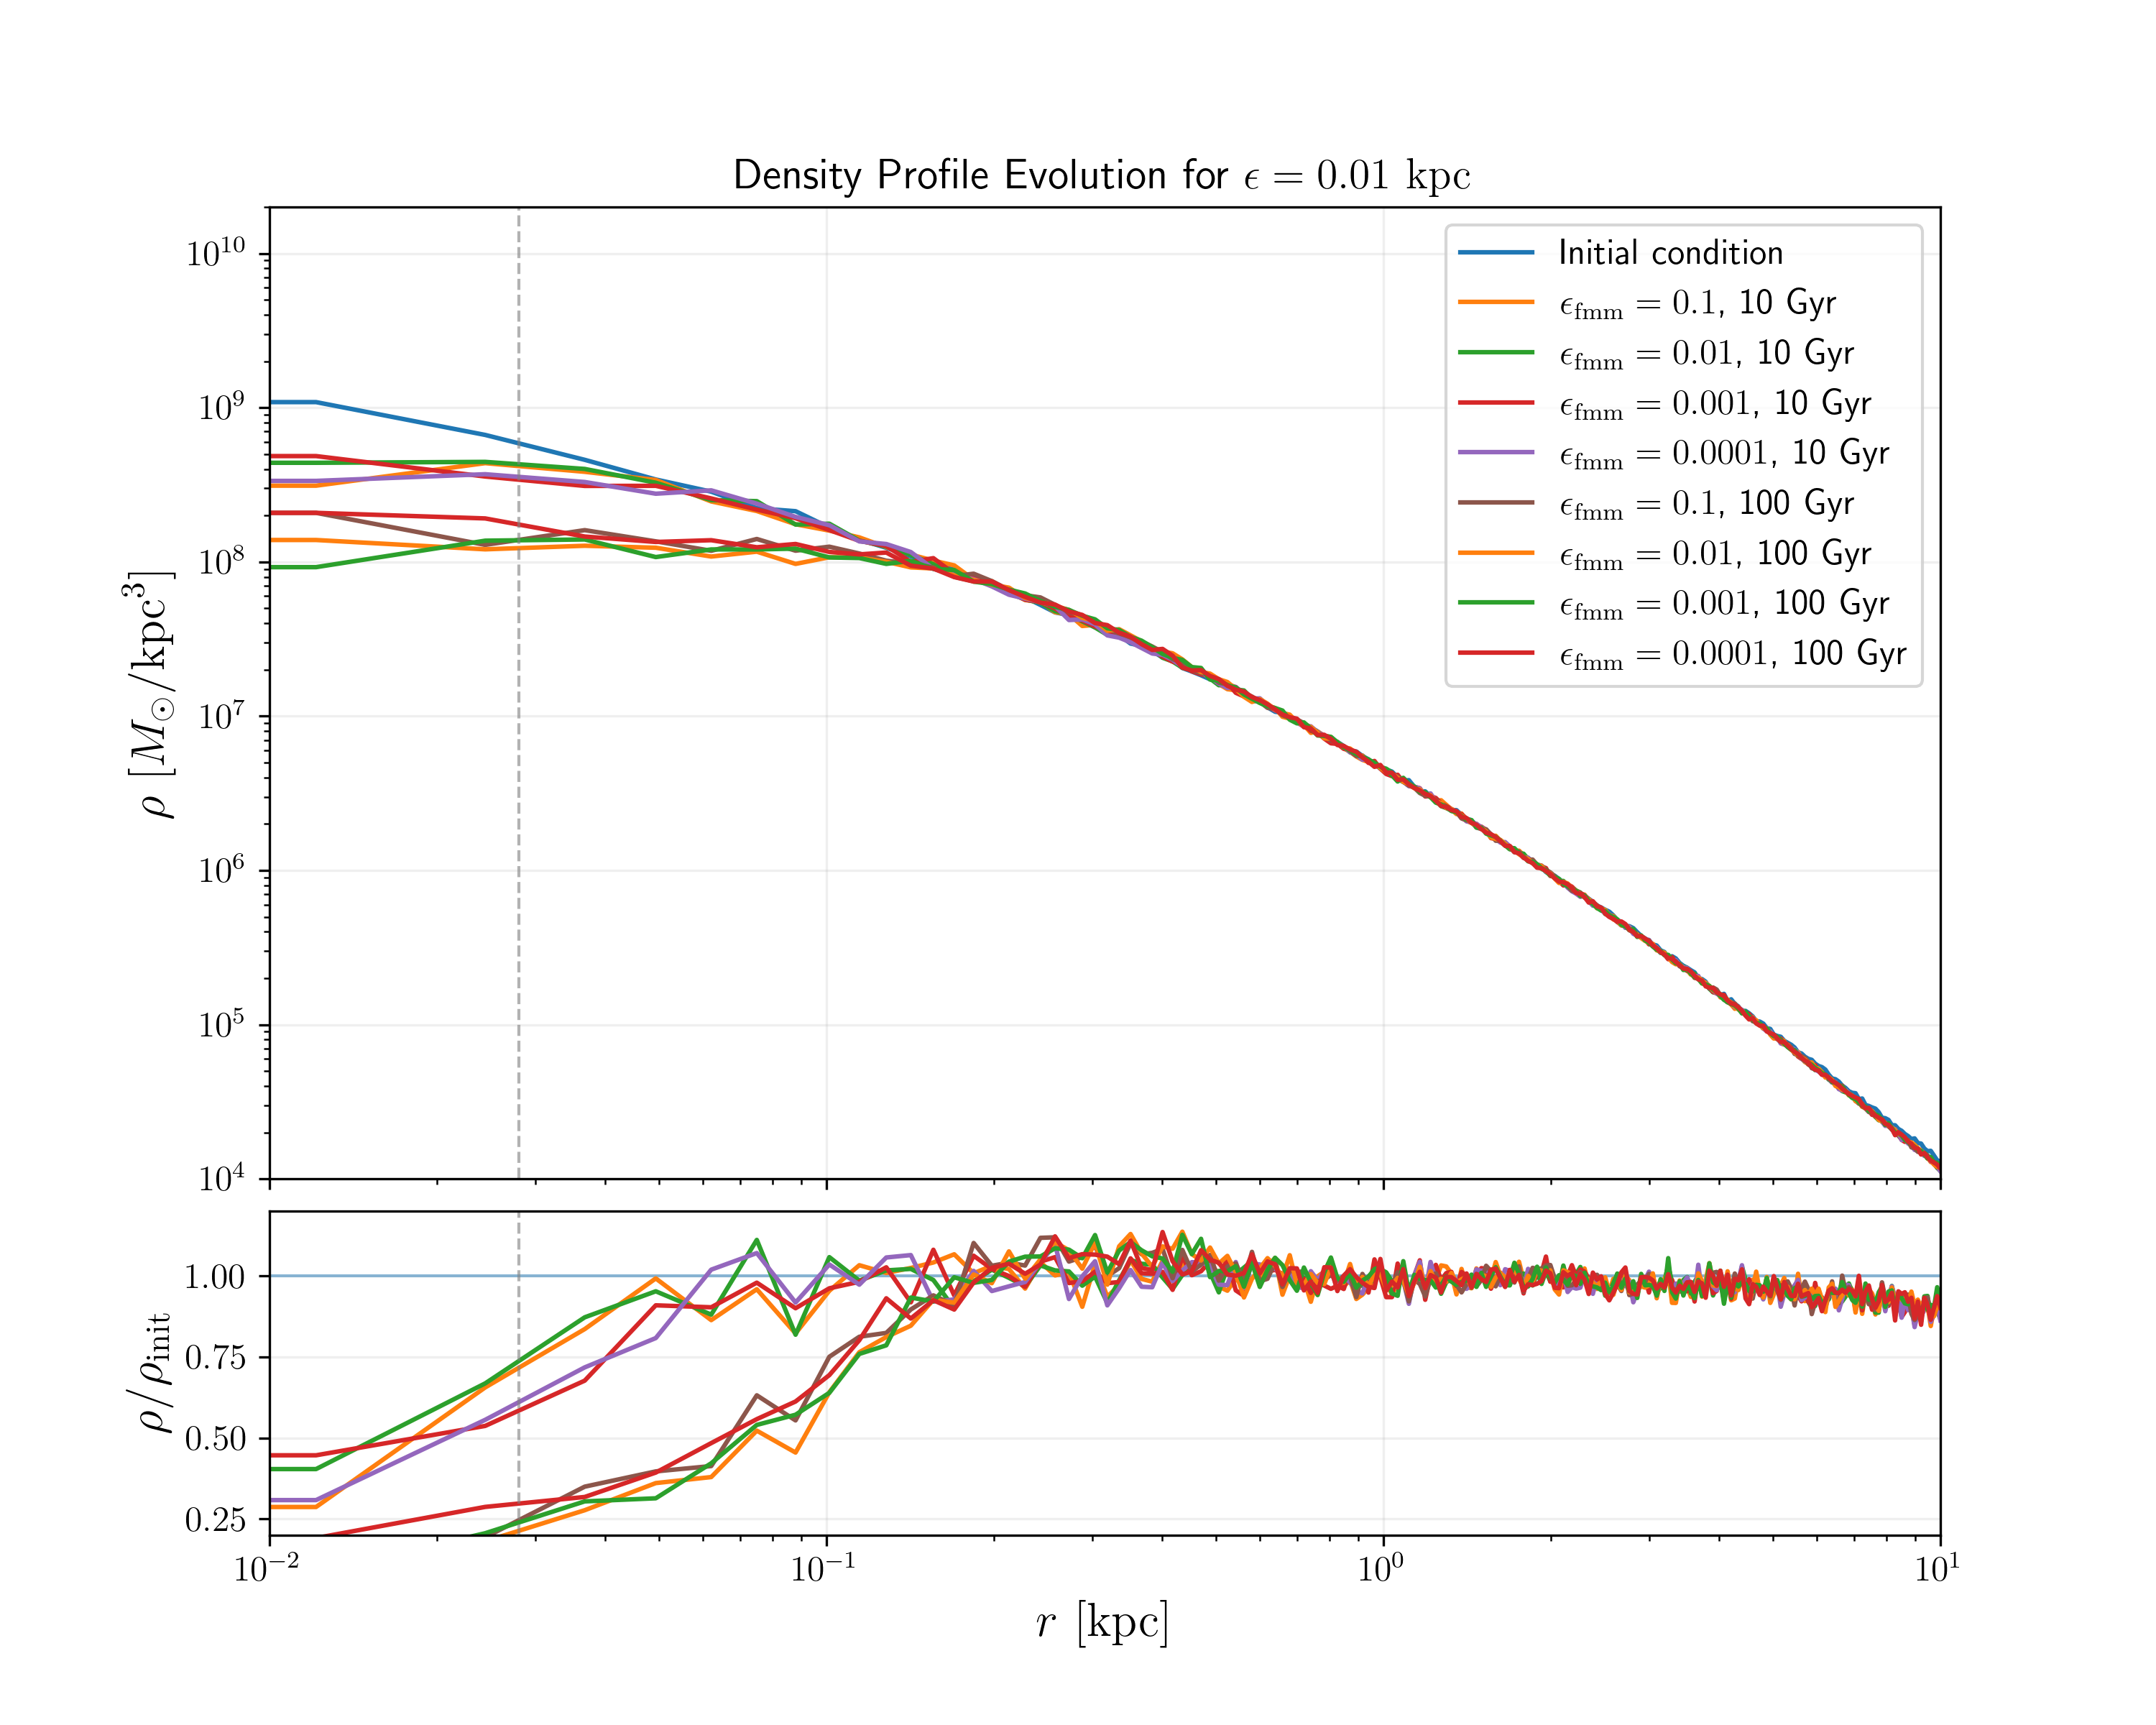
\includegraphics[width=0.95\textwidth]{comp_eps.png}
    \caption{Comparison of $\epsilon_{\mathrm{fmm}}$ sensitivity: baseline 0.001 versus test values 0.0001, 0.01, 0.1.}
\end{figure}

\clearpage
\section*{MAC}

\begin{figure}[H]
    \centering
    \begin{minipage}{\textwidth}
        \centering
        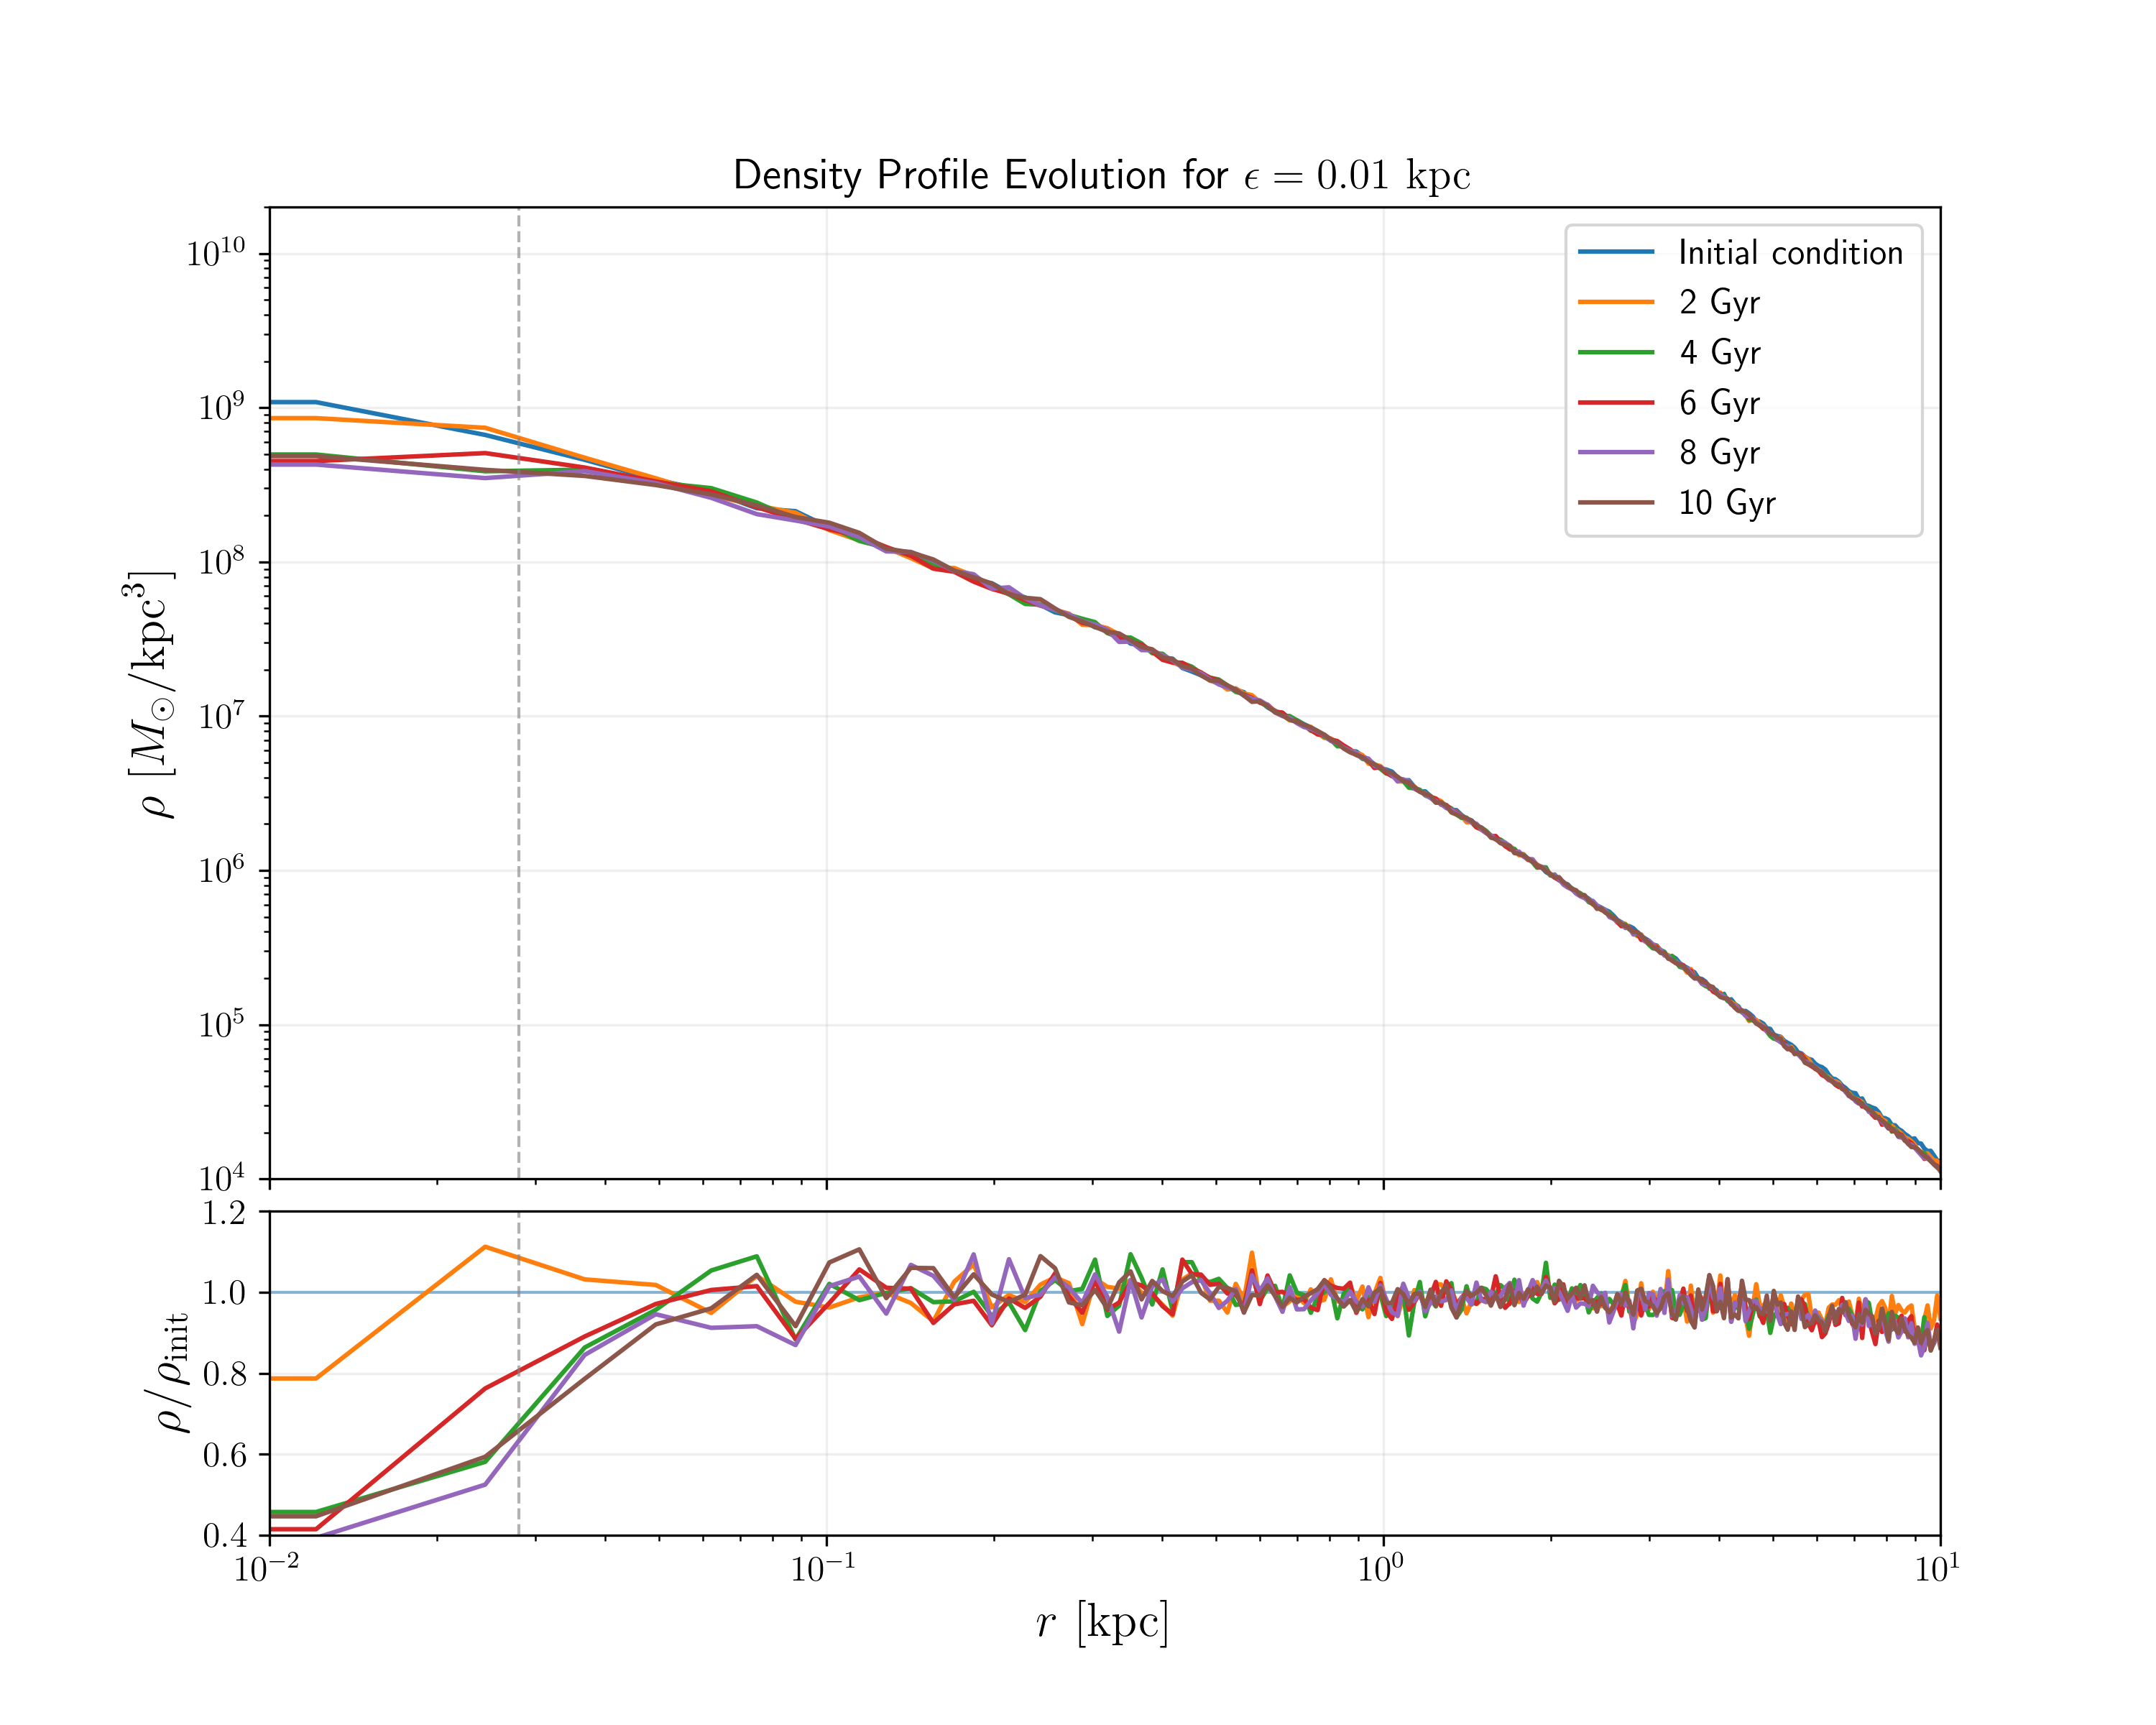
\includegraphics[width=0.48\textwidth]{density_evo_mac_10.png}
        \hfill
        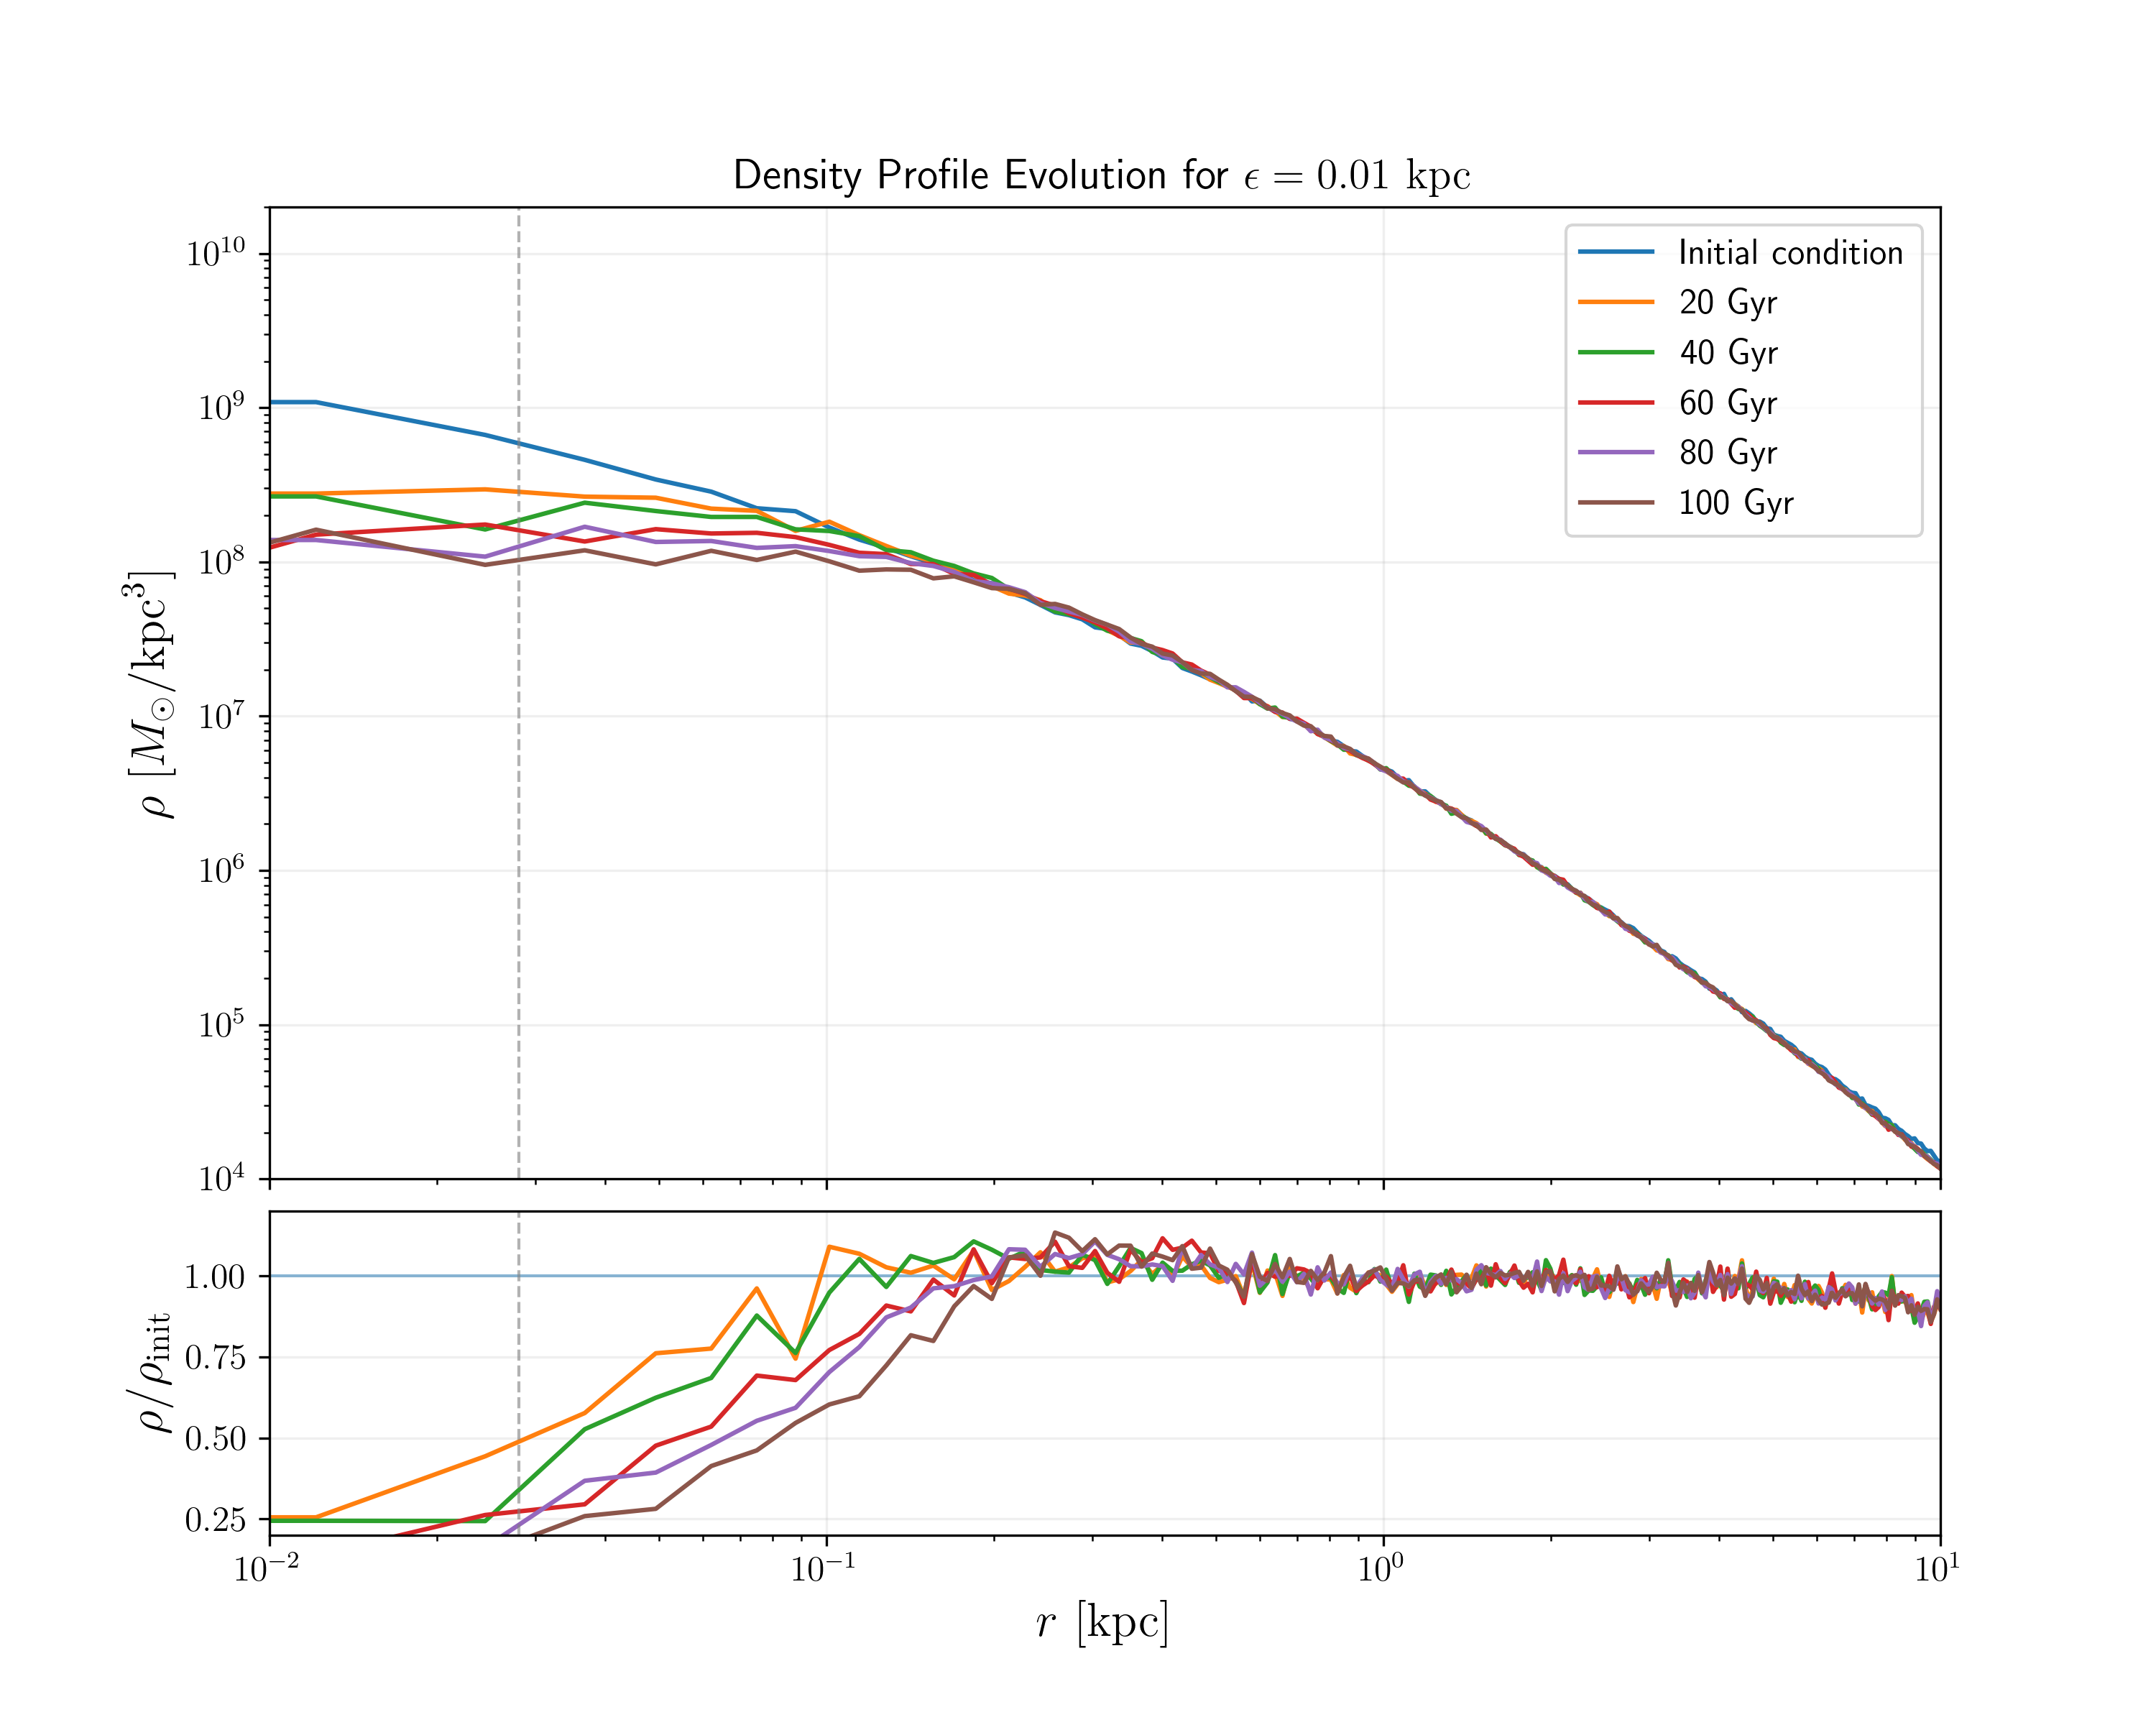
\includegraphics[width=0.48\textwidth]{density_evo_mac_100.png}
    \end{minipage}
    \caption{Density evolution for MAC method. Left: adaptive MAC at step 10; Right: adaptive MAC at step 100.}
\end{figure}

\begin{figure}[H]
    \centering
    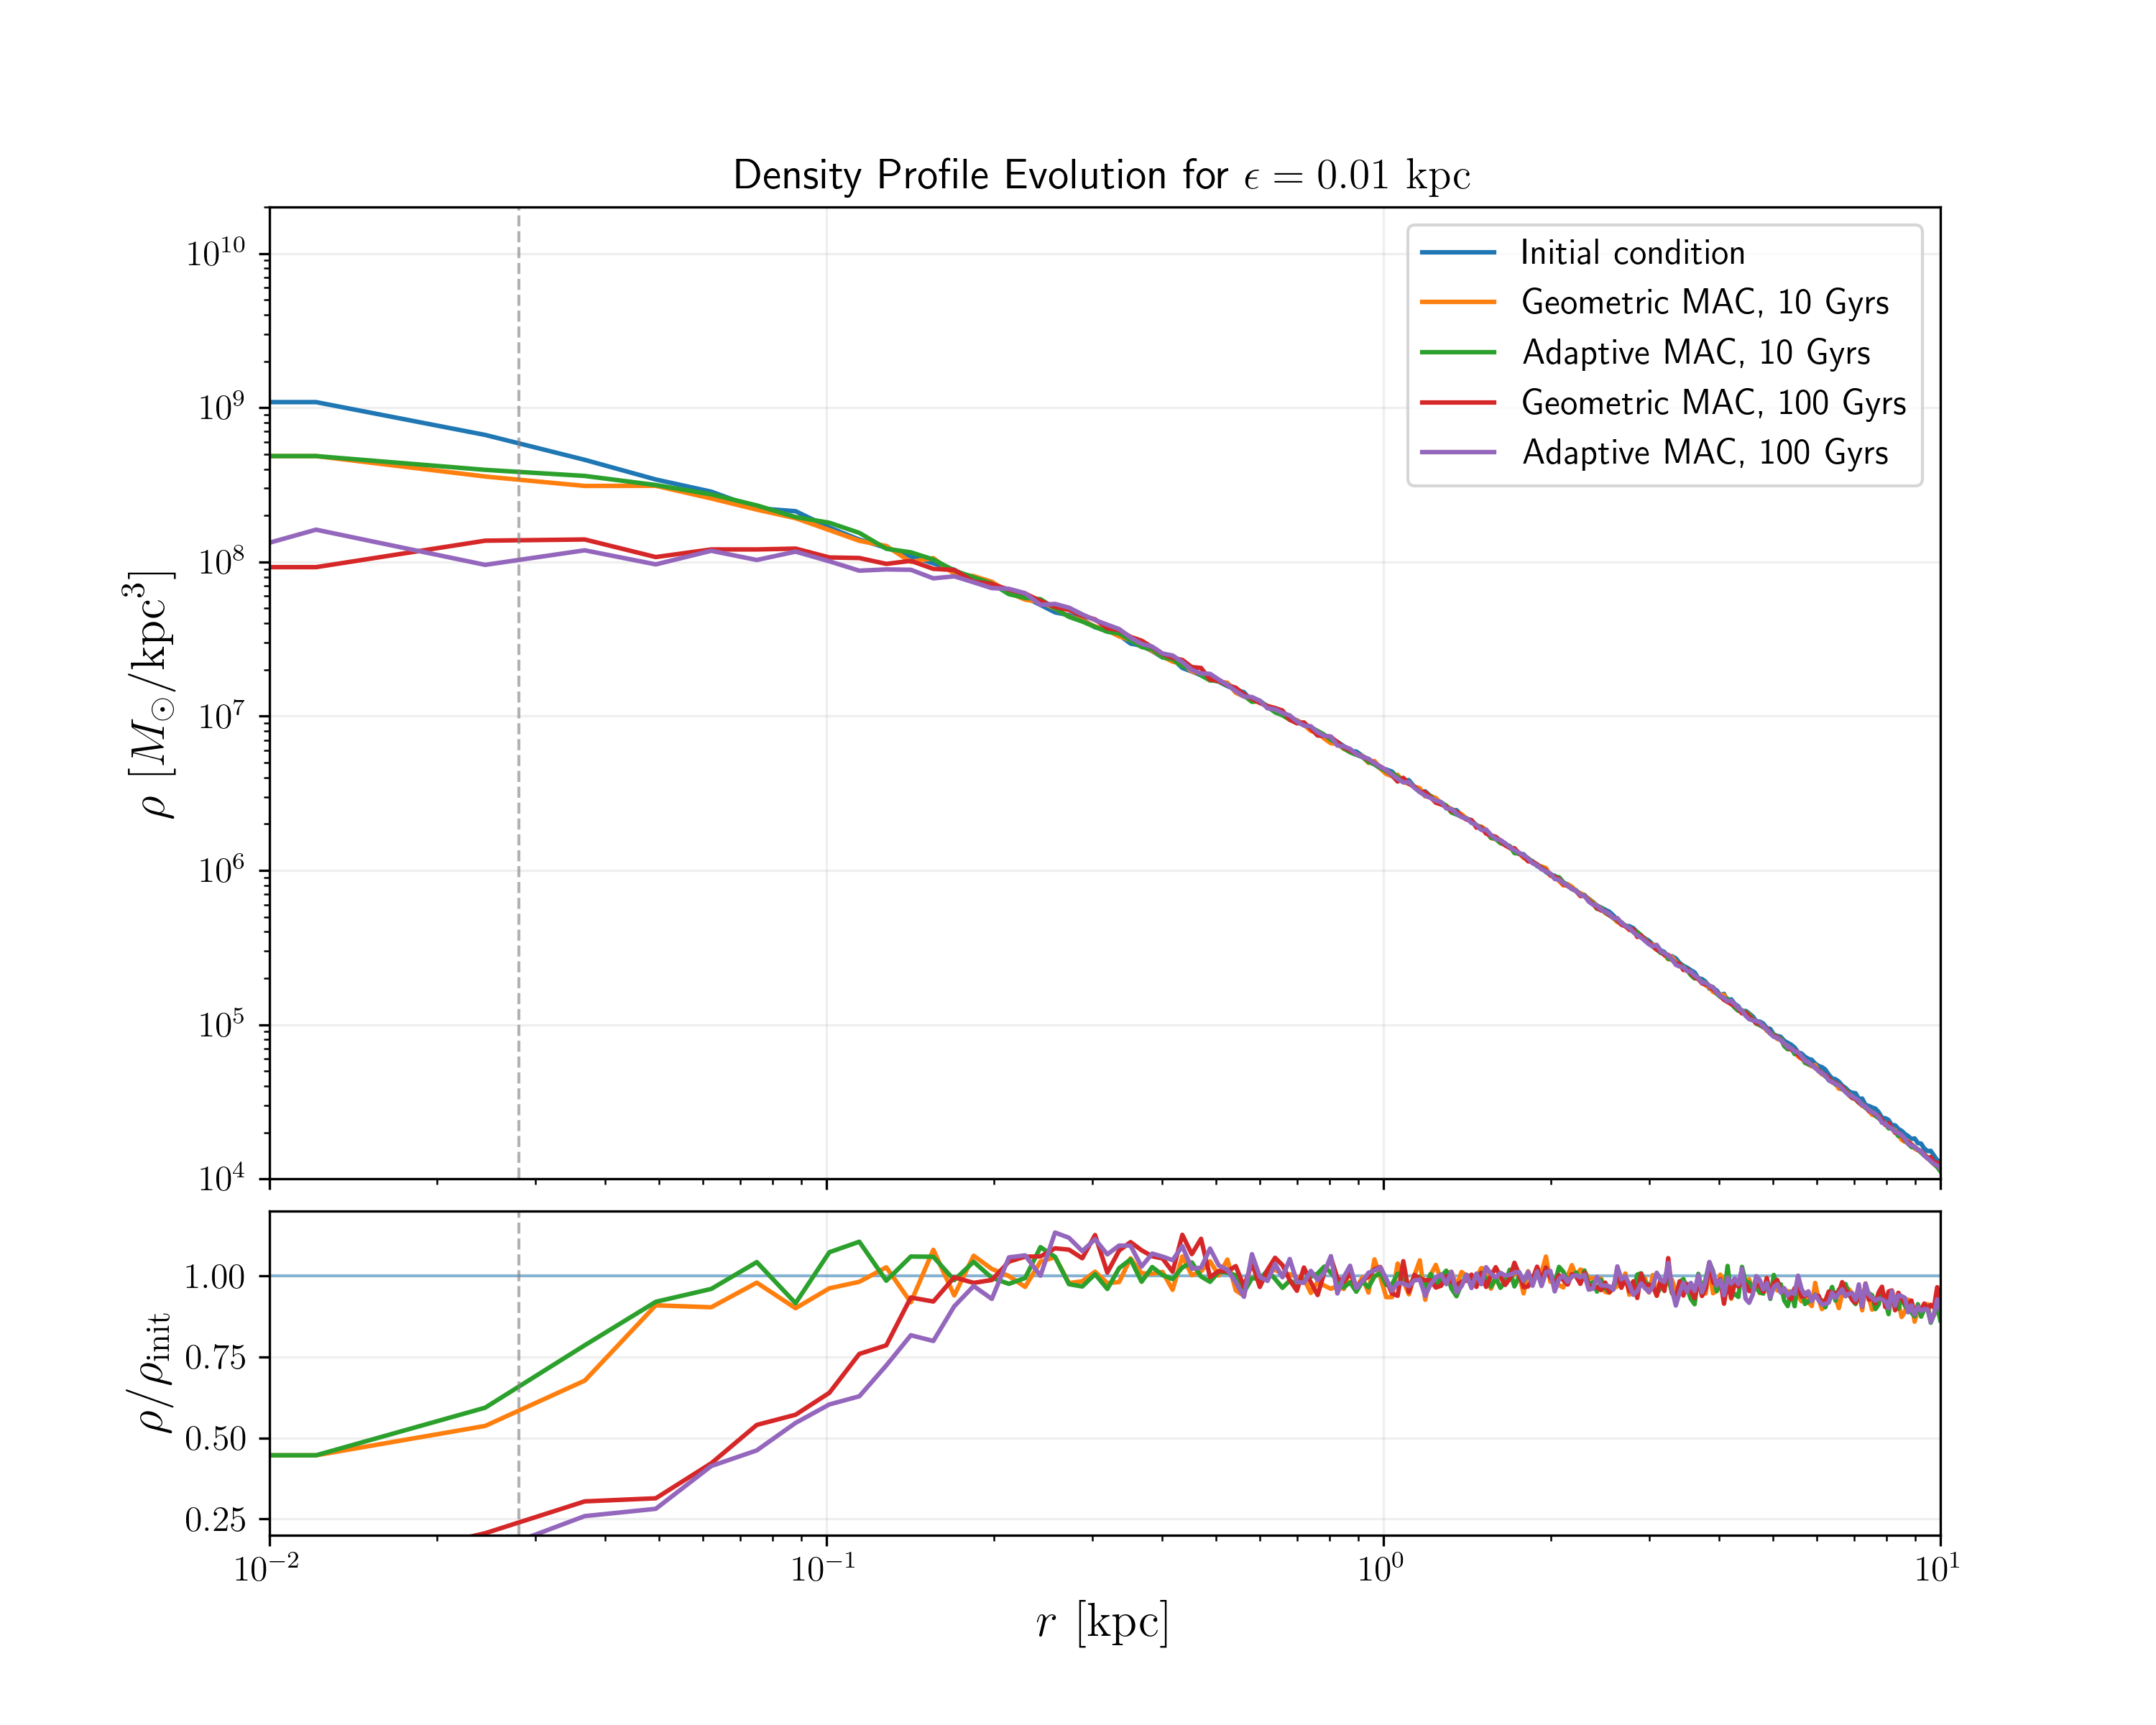
\includegraphics[width=0.95\textwidth]{comp_mac.png}
    \caption{Comparison of MAC method sensitivity: baseline (geometric) versus adaptive MAC.}
\end{figure}

\clearpage
\section*{$\theta_{\mathrm{cr}}$}

\begin{figure}[H]
    \centering
    \begin{minipage}{\textwidth}
        \centering
        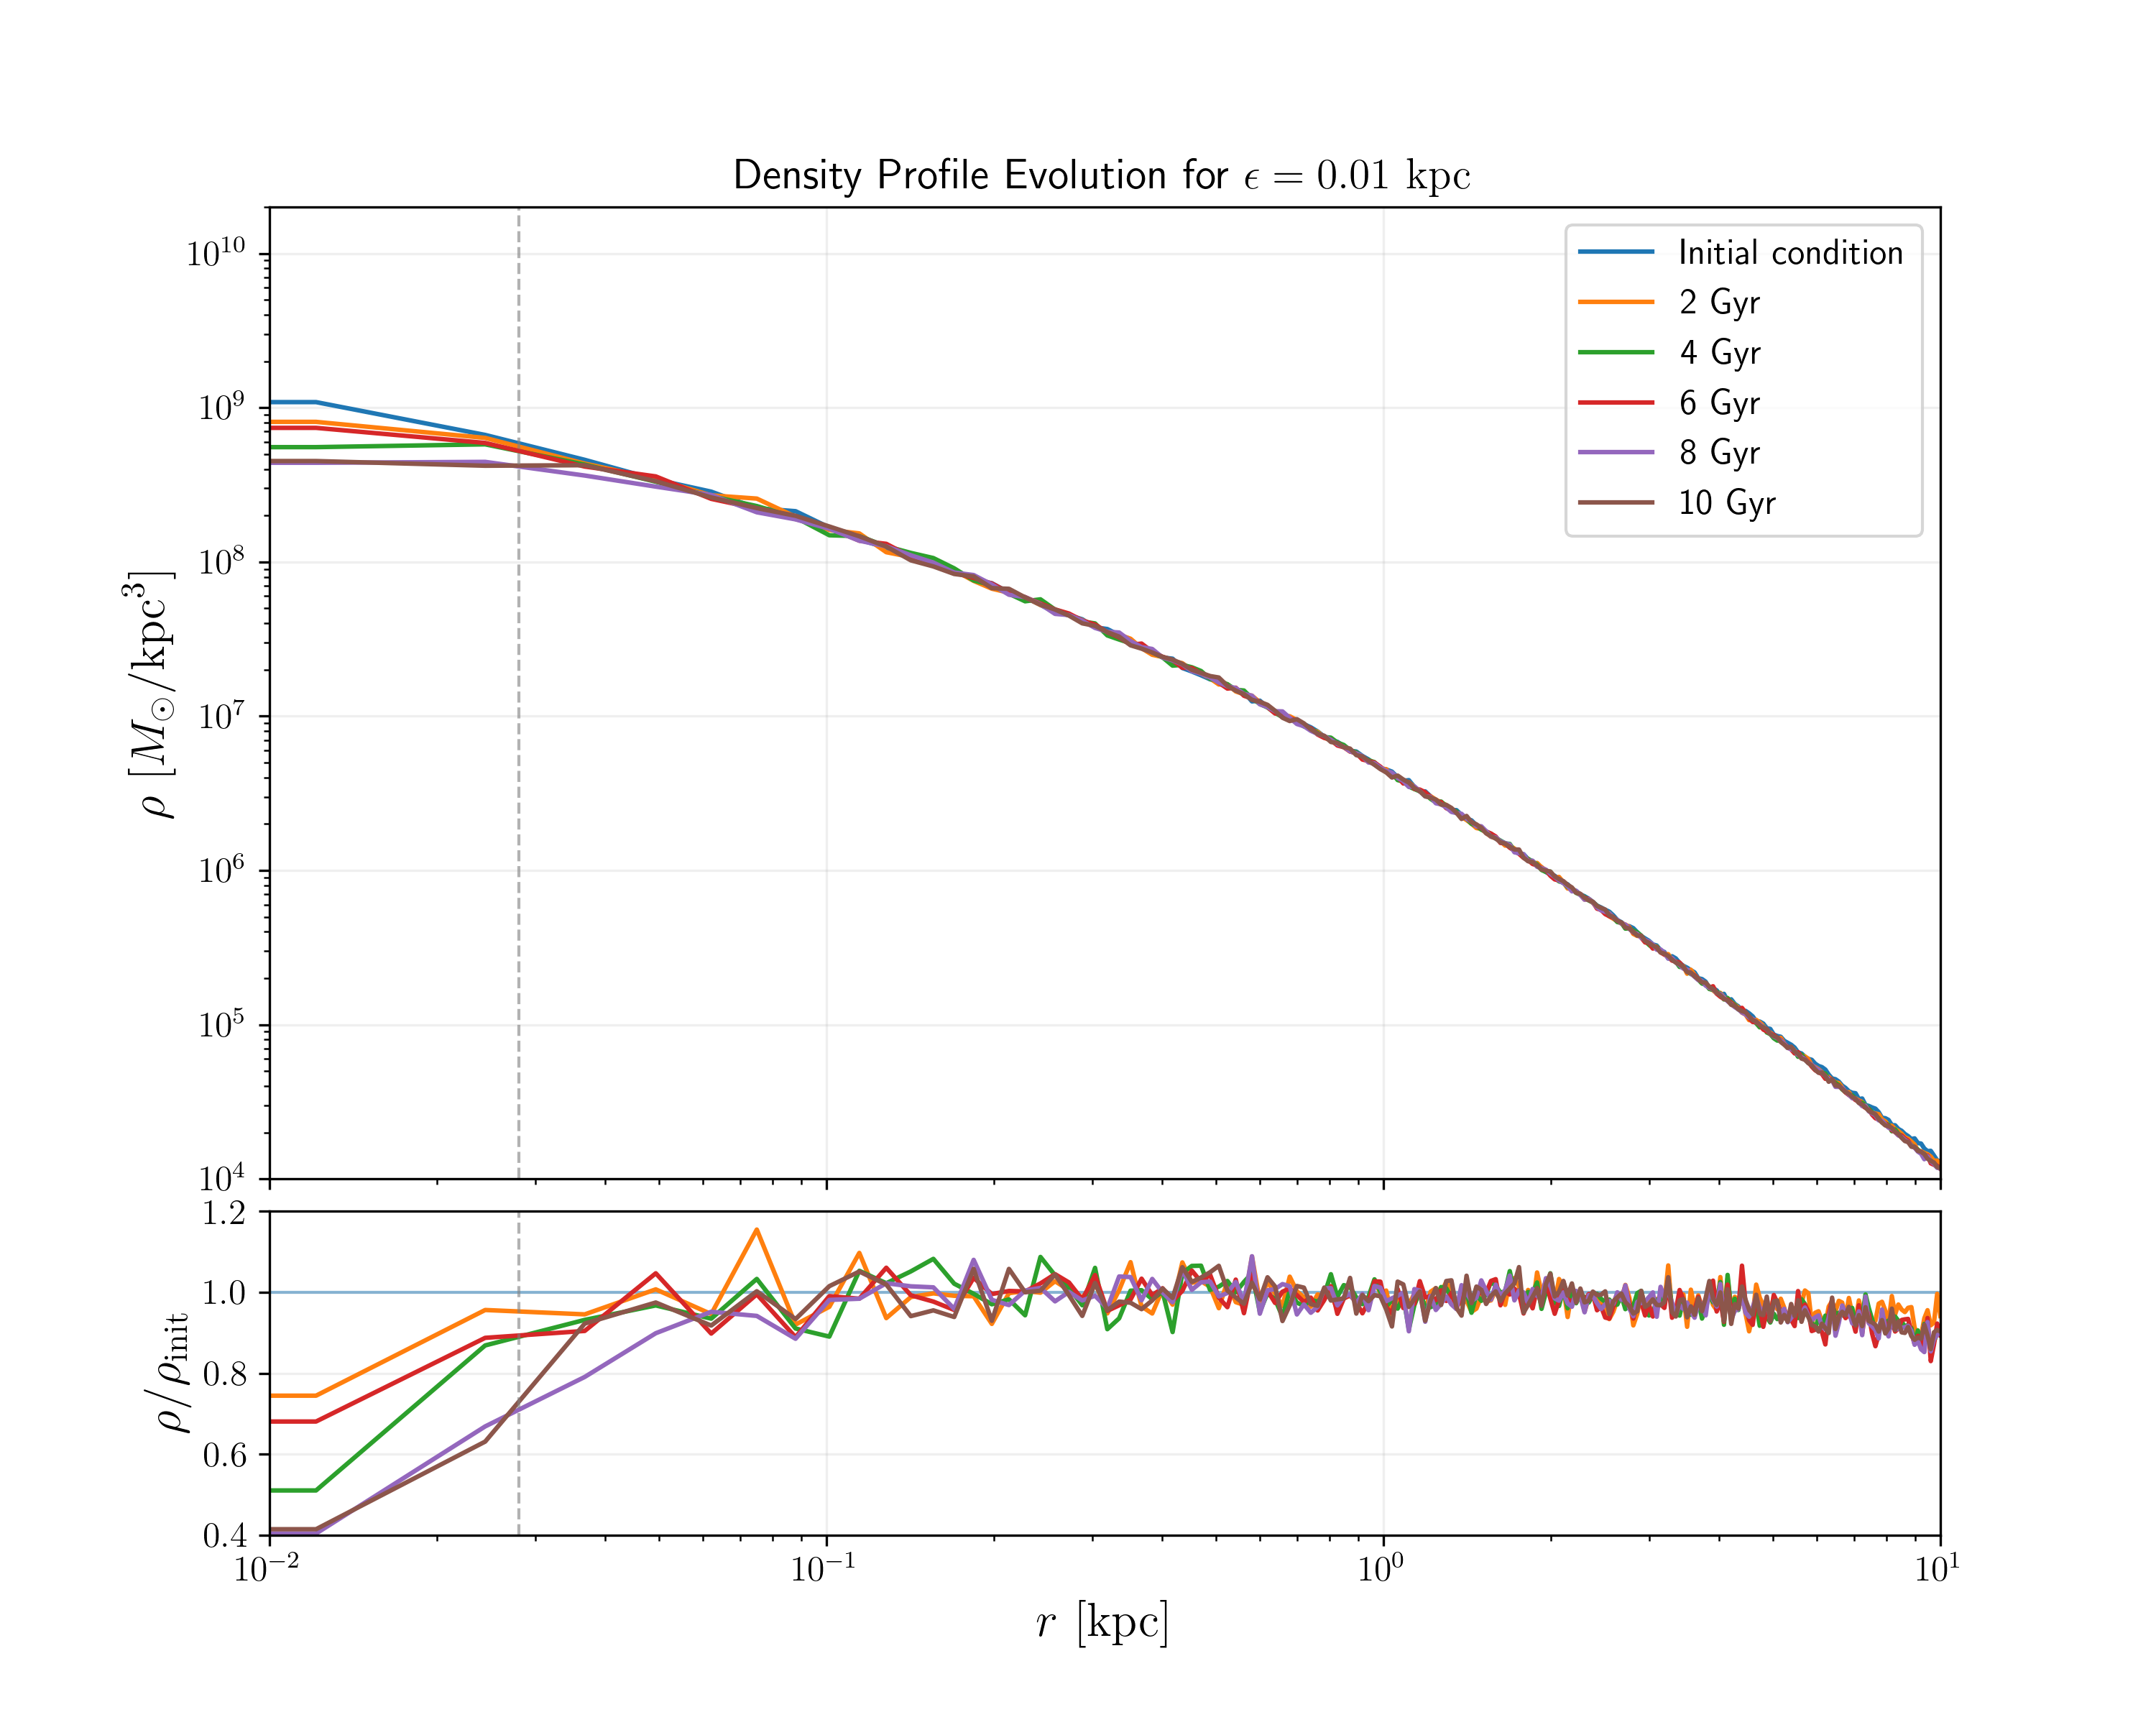
\includegraphics[width=0.48\textwidth]{density_evo_theta_10.png}
        \hfill
        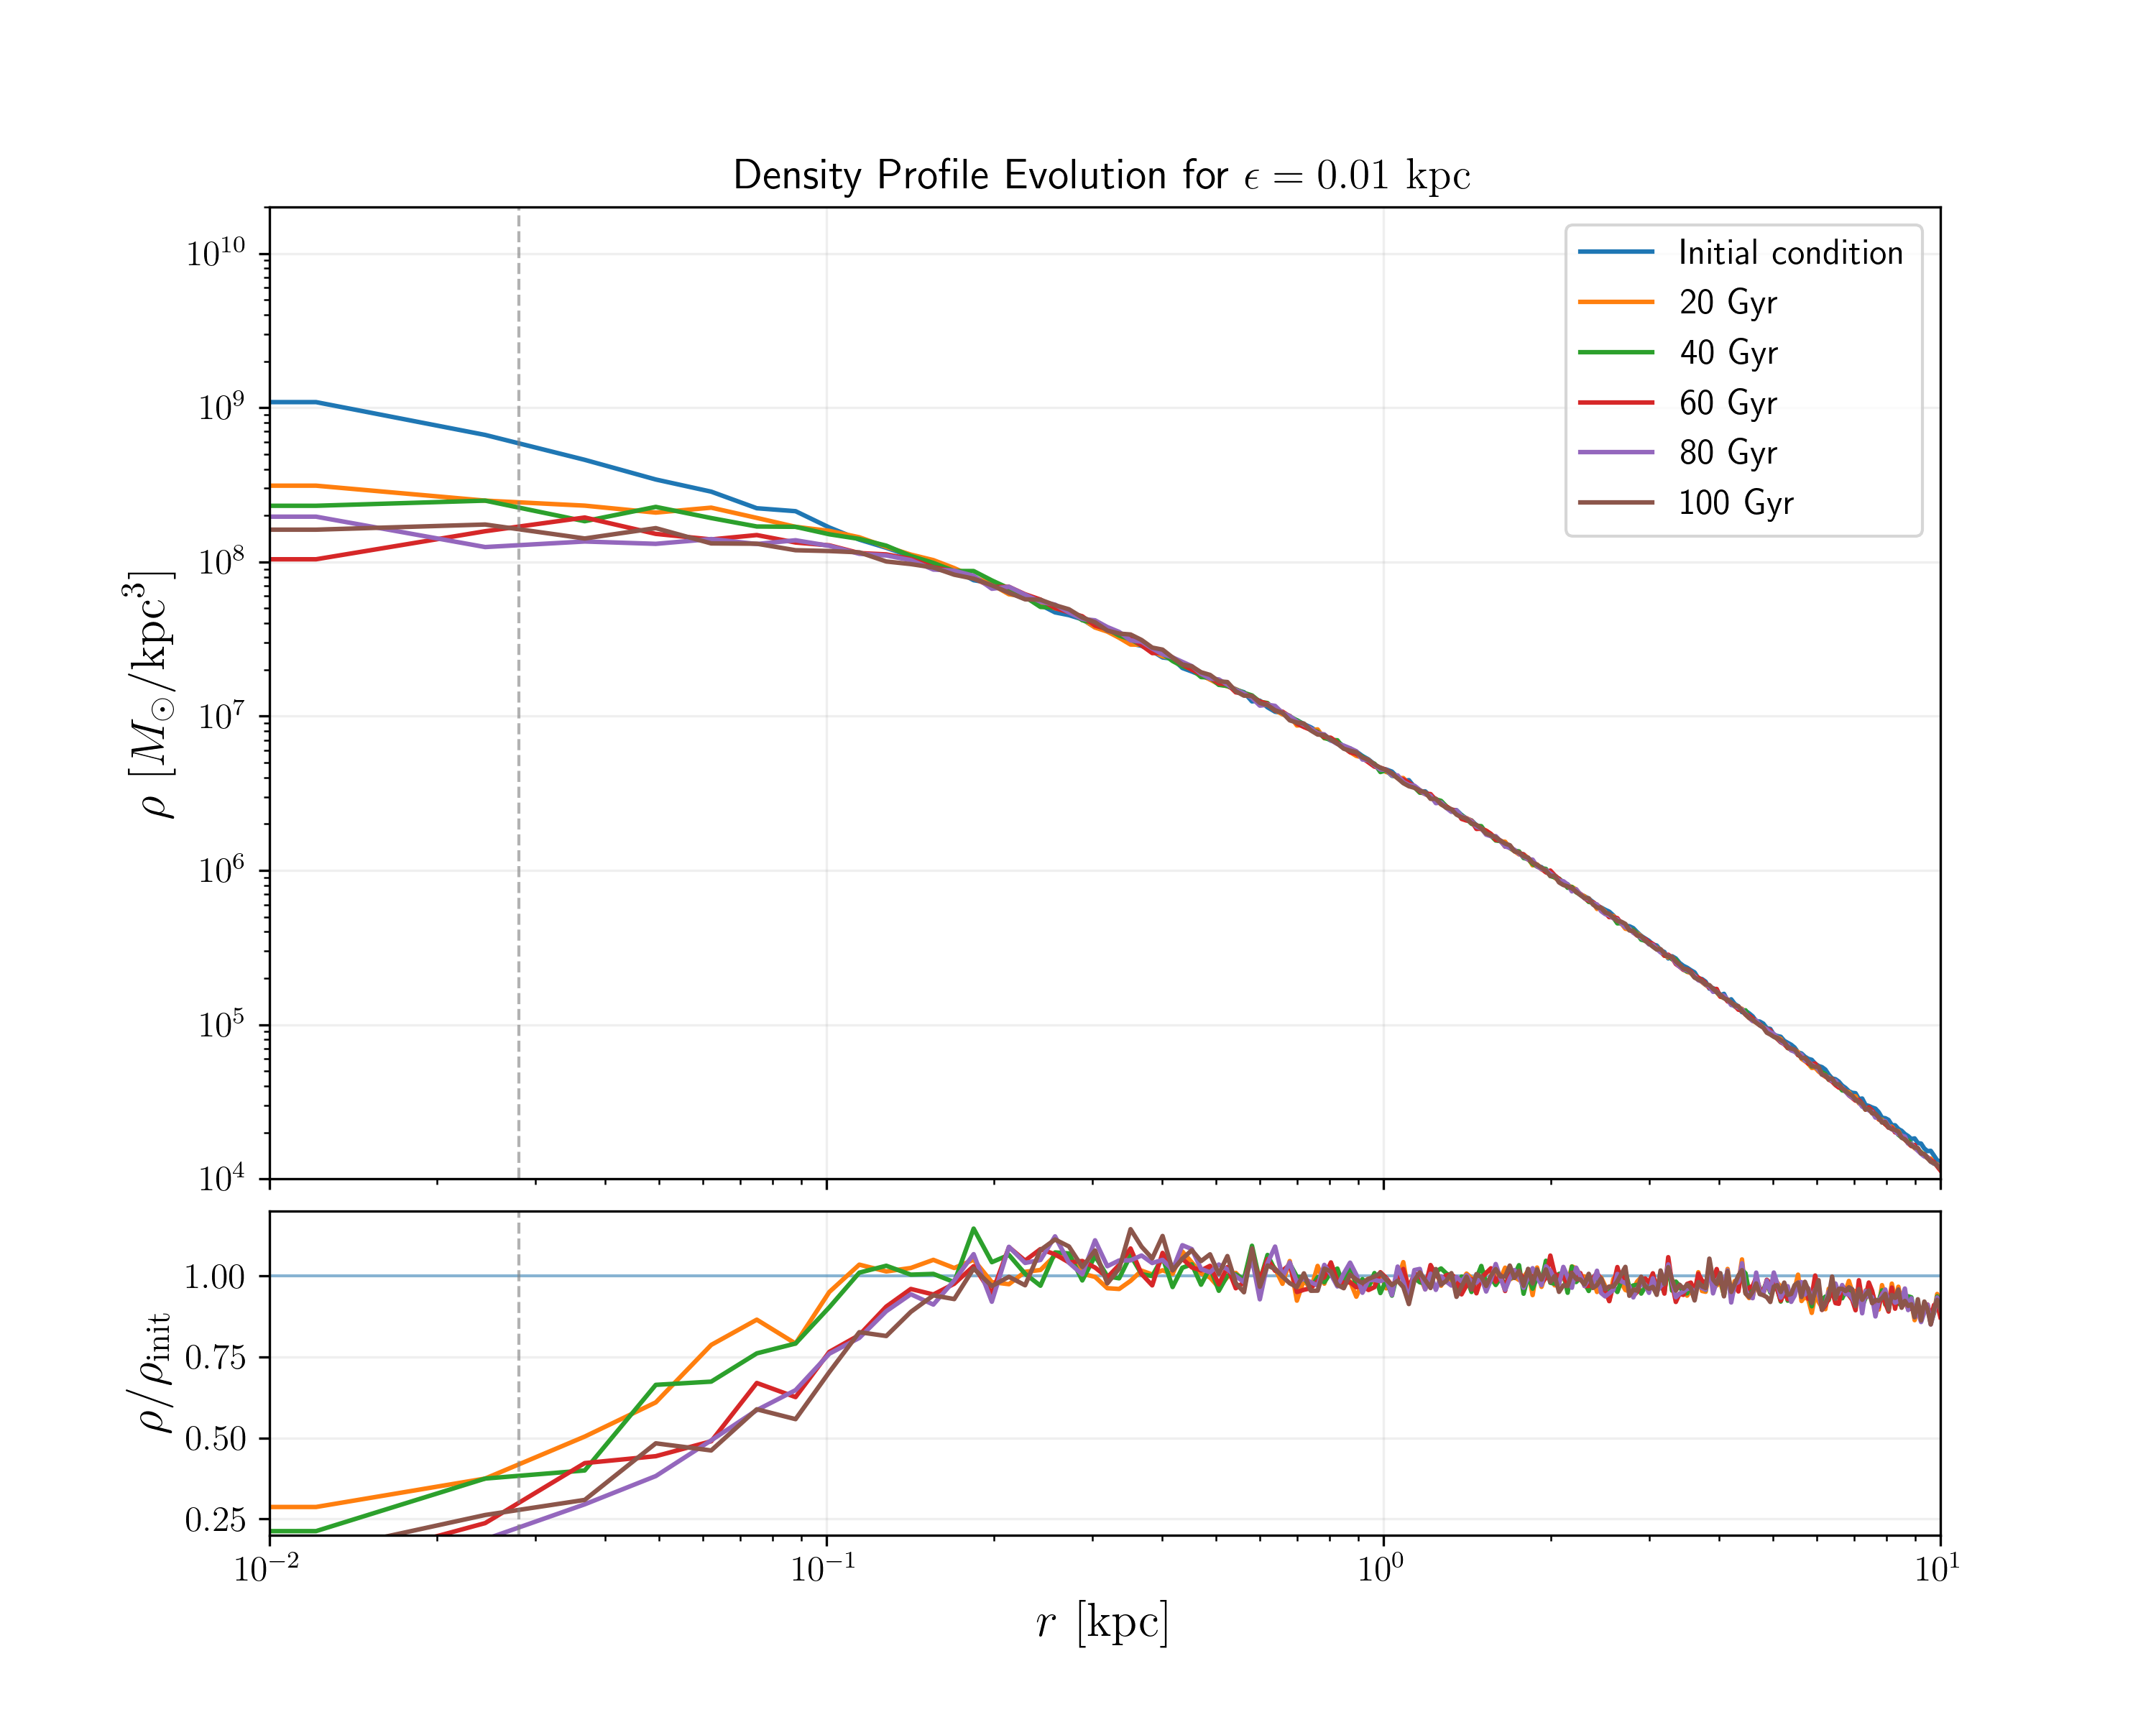
\includegraphics[width=0.48\textwidth]{density_evo_theta_100.png}
    \end{minipage}
    \caption{Density evolution for $\theta_{\mathrm{cr}}$ test. Left: $\theta_{\mathrm{cr}} = 0.5$ at step 10; Right: $\theta_{\mathrm{cr}} = 0.5$ at step 100.}
\end{figure}

\begin{figure}[H]
    \centering
    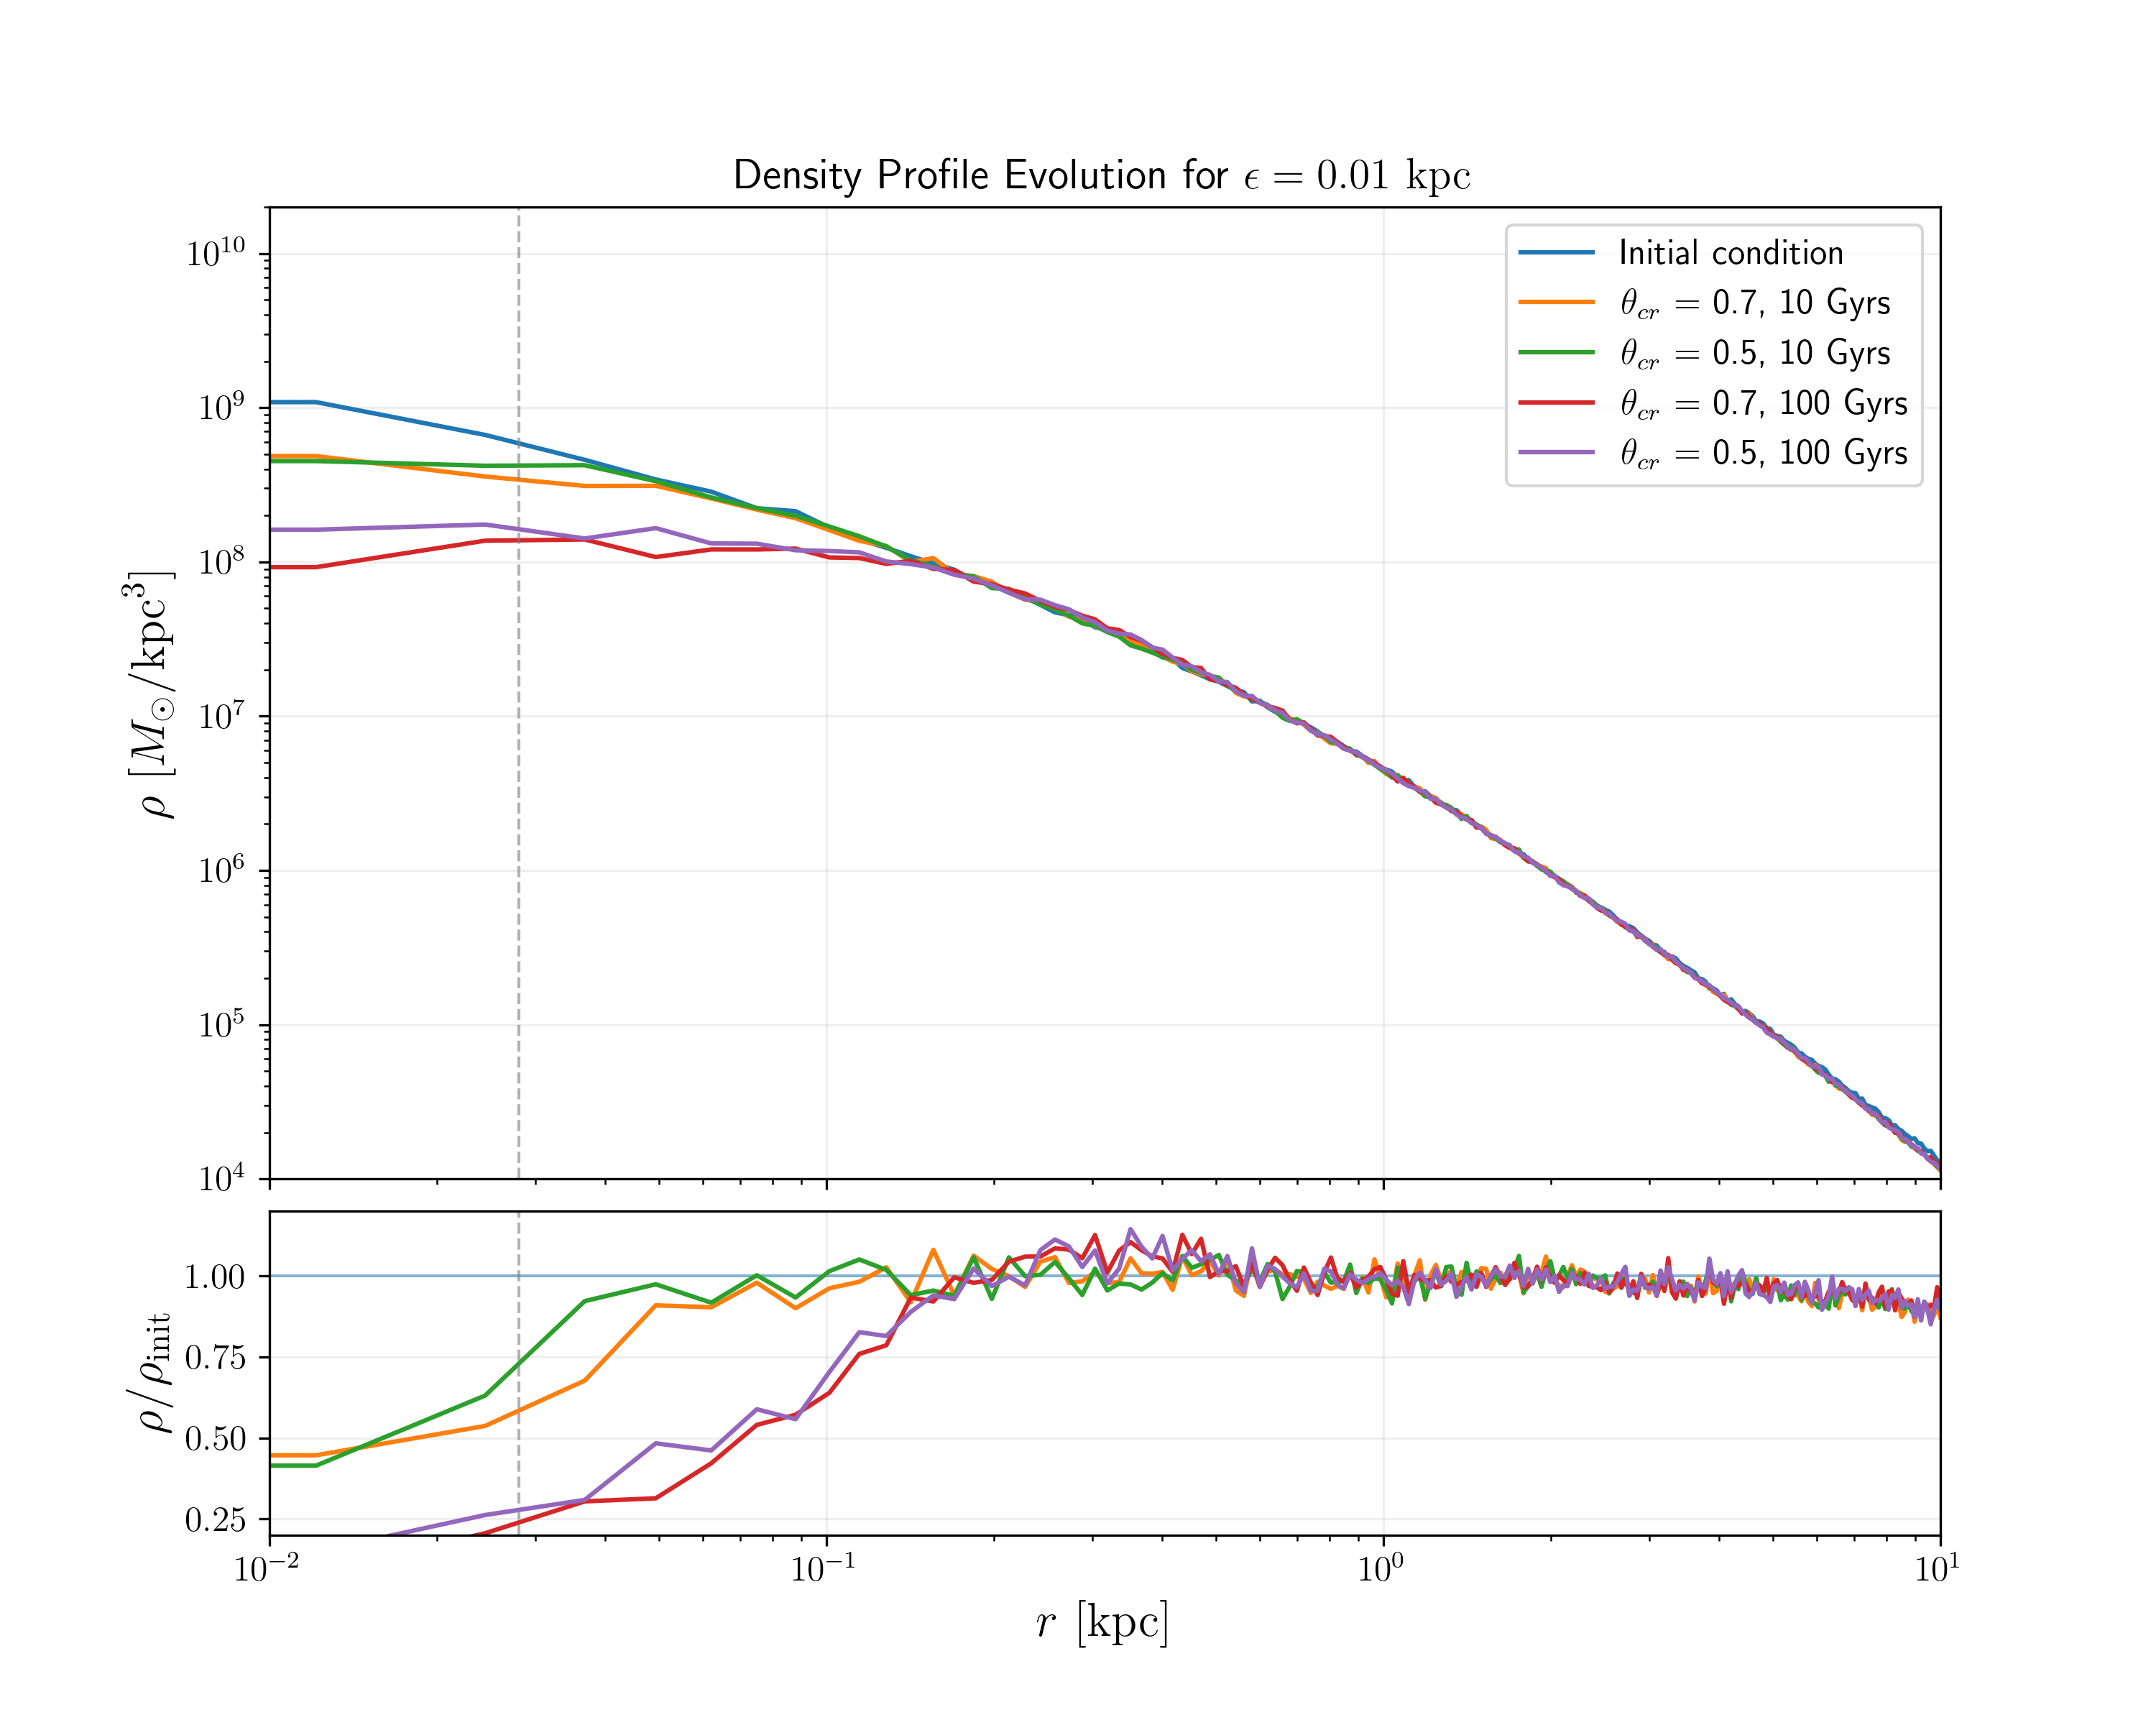
\includegraphics[width=0.95\textwidth]{comp_theta.png}
    \caption{Comparison of $\theta_{\mathrm{cr}}$ sensitivity: baseline 0.7 versus test value 0.5.}
\end{figure}

\clearpage
\section*{$\eta$ (timestep)}

\begin{figure}[H]
    \centering
    \begin{minipage}{\textwidth}
        \centering
        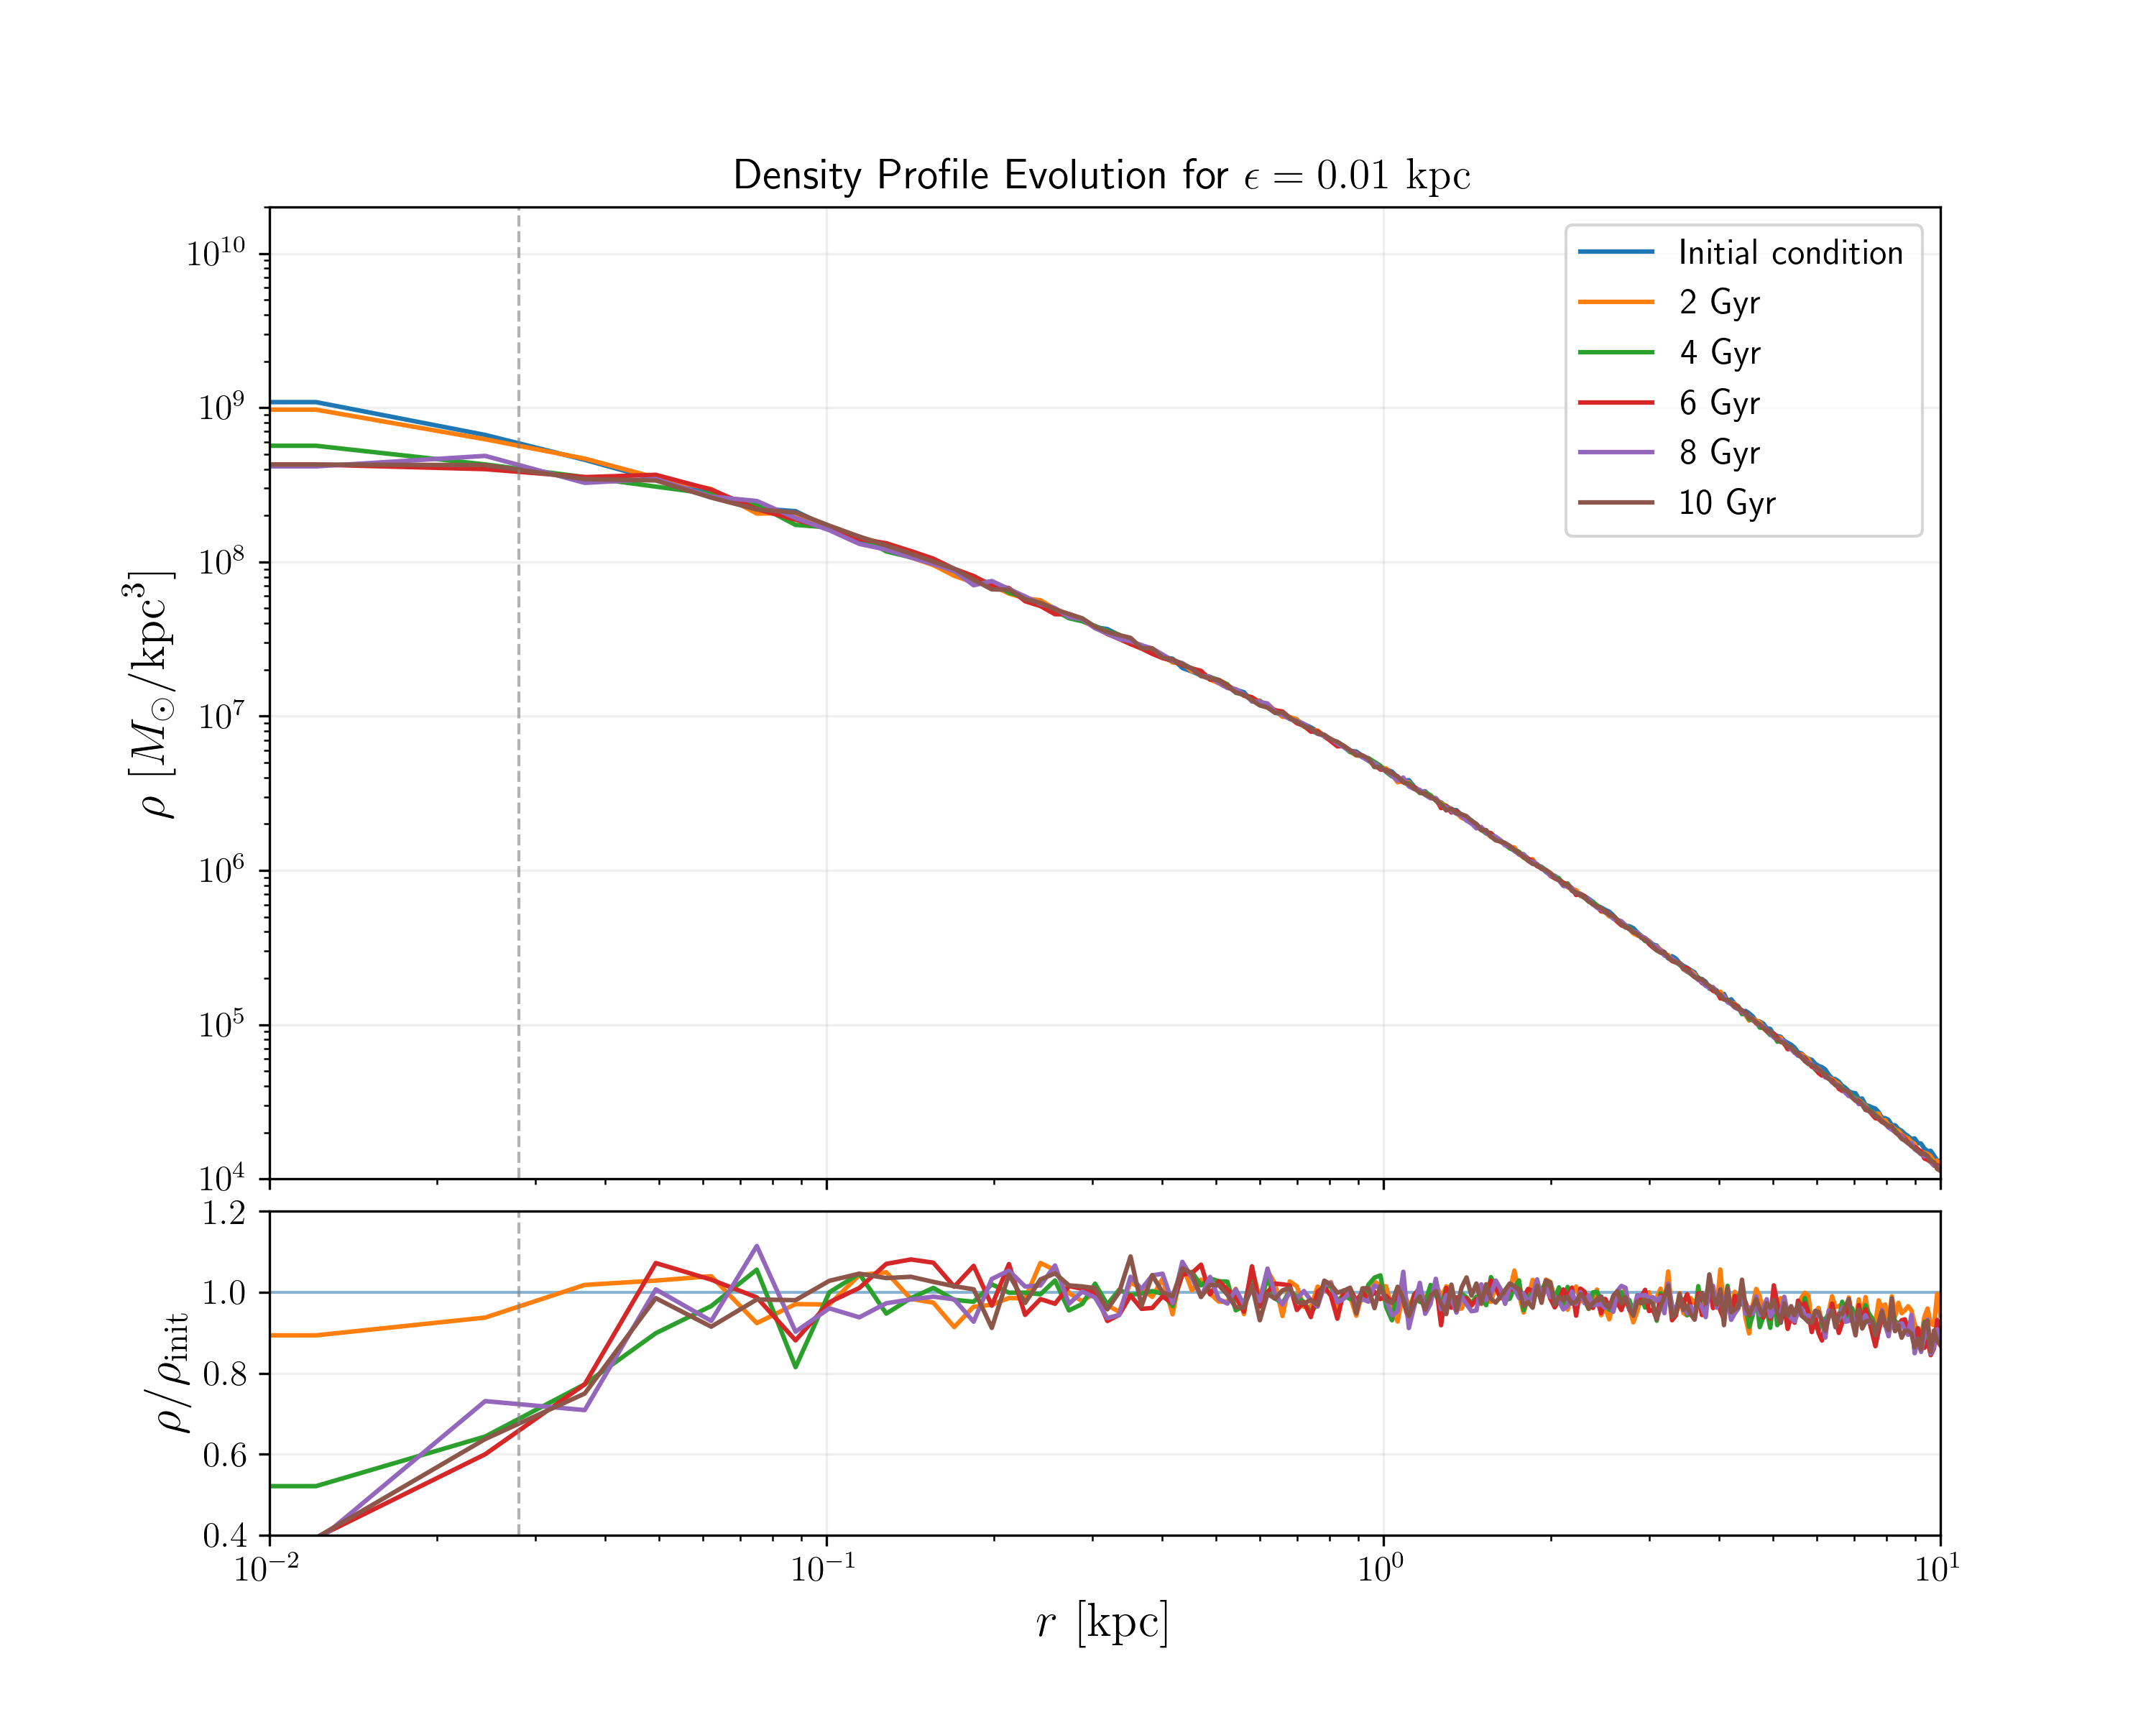
\includegraphics[width=0.48\textwidth]{density_evo_timestep01_10.png}
        \hfill
        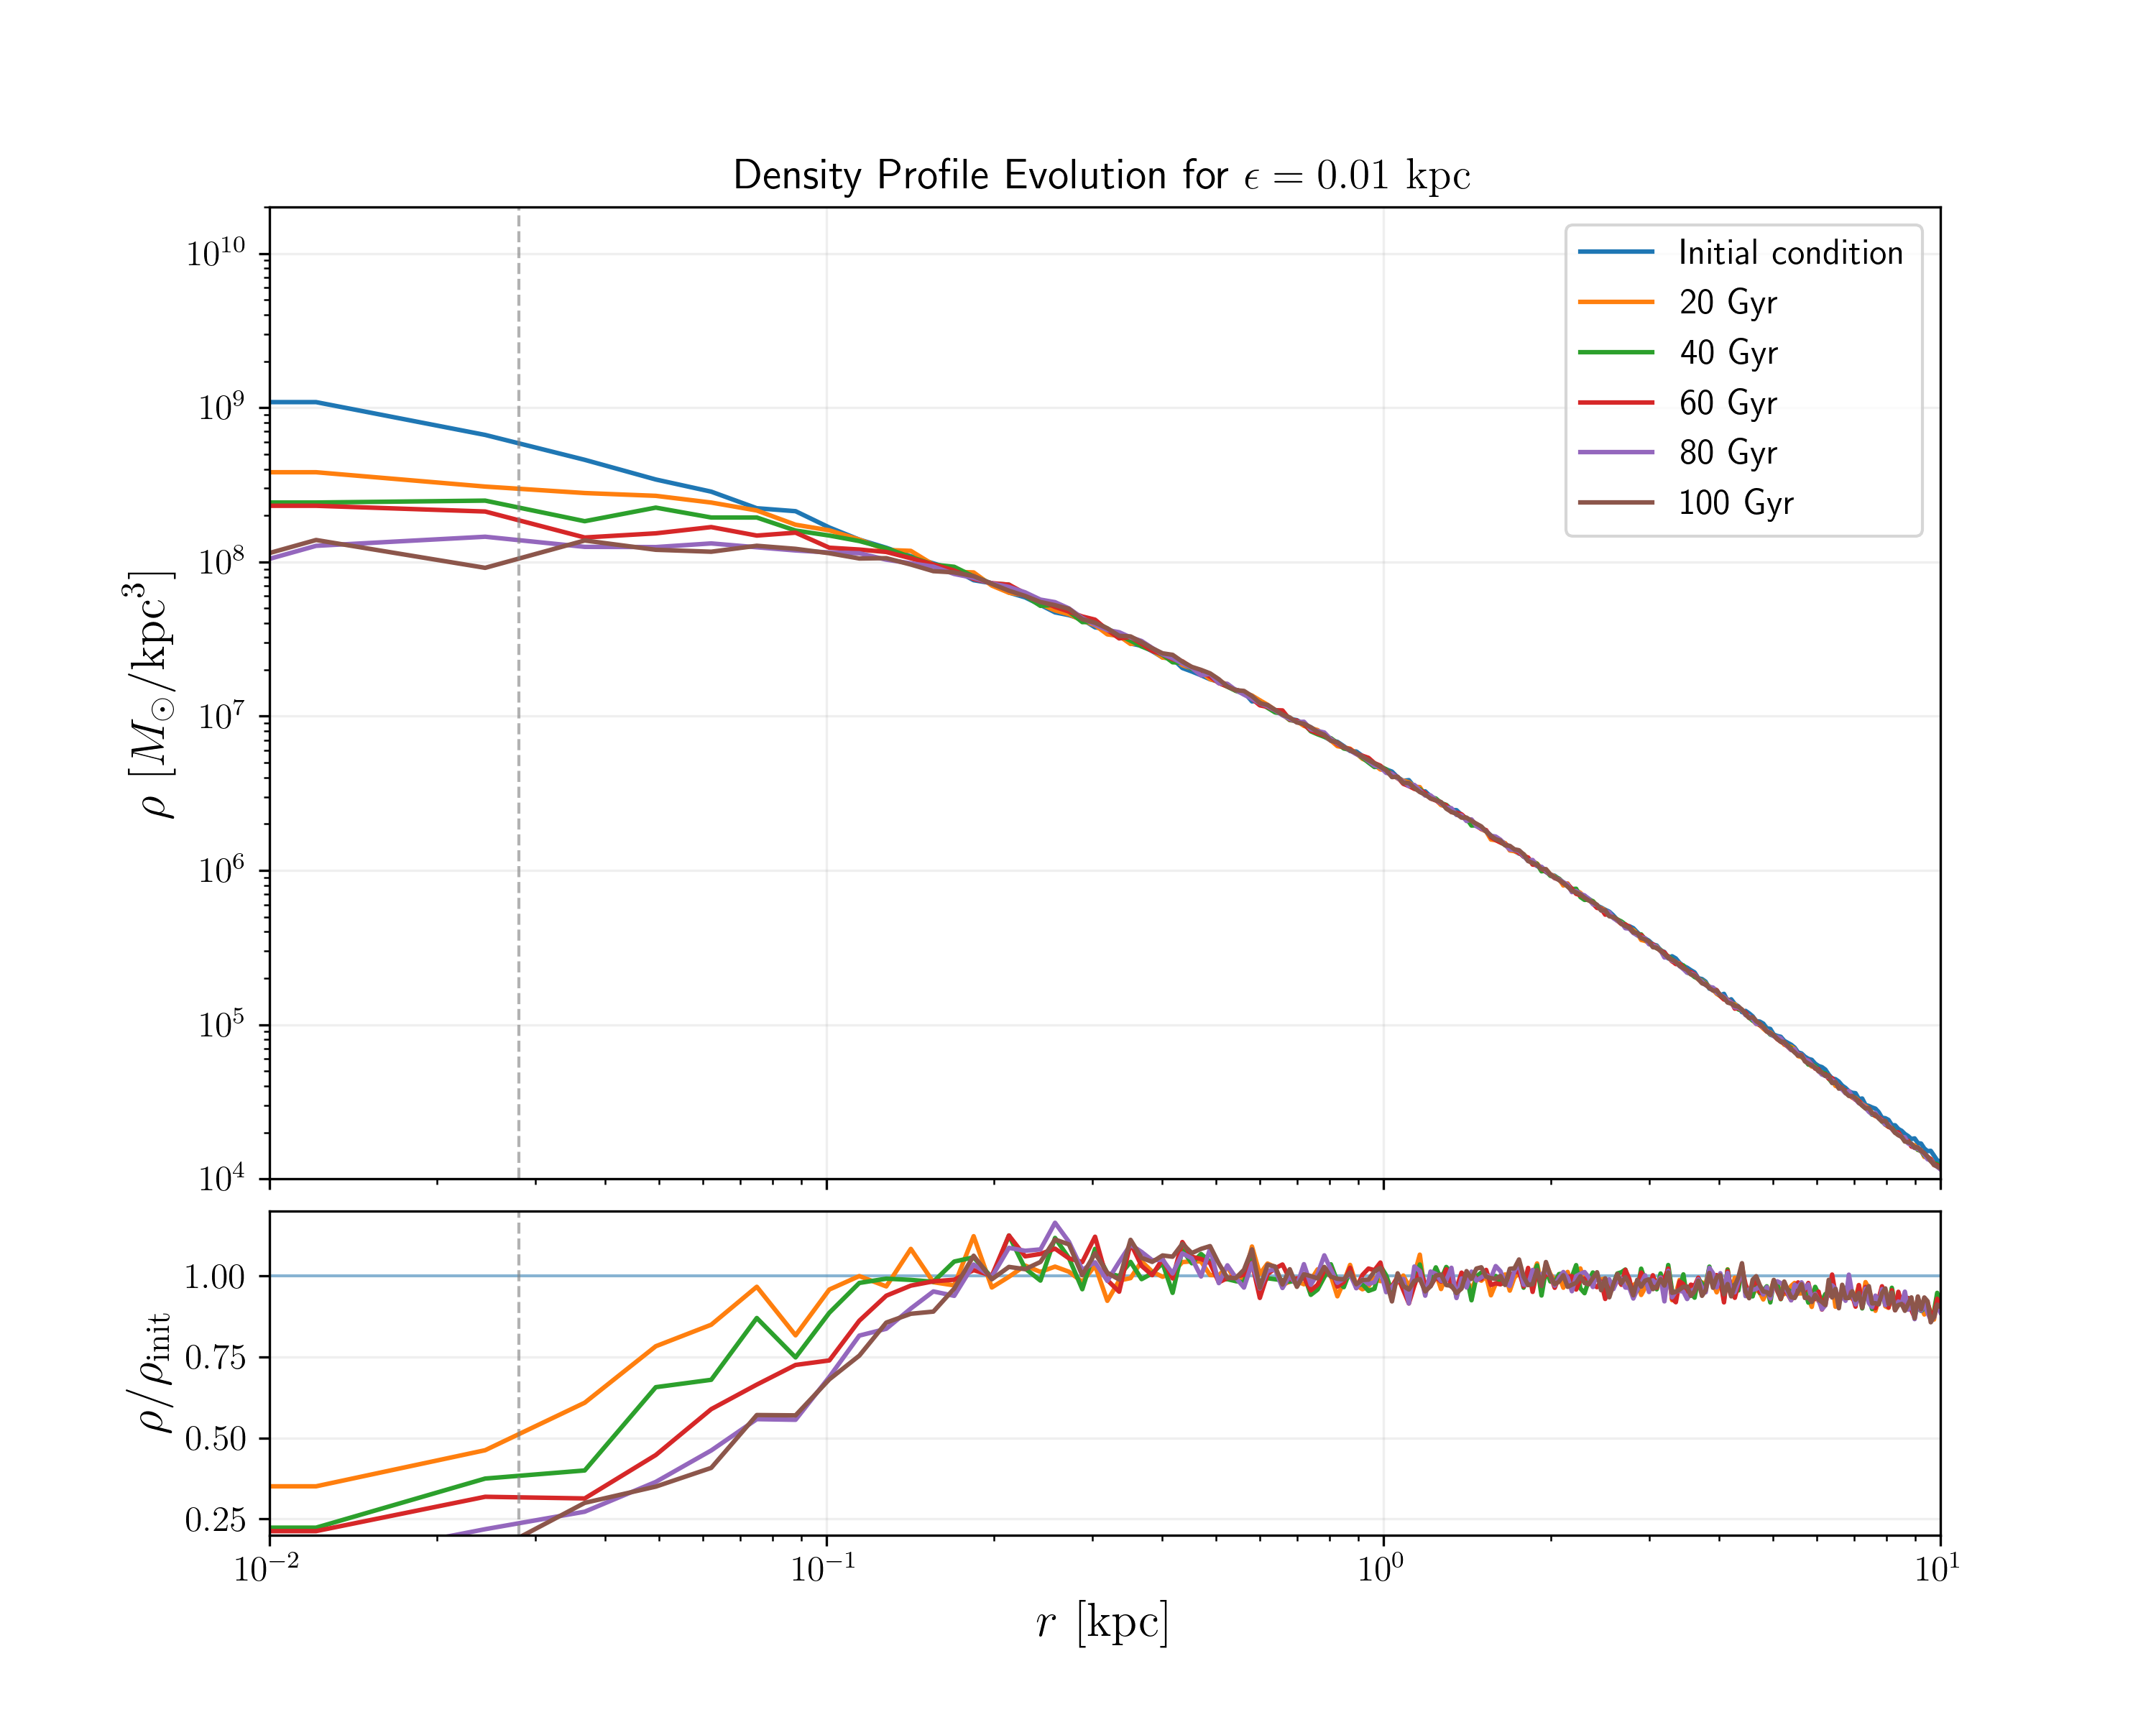
\includegraphics[width=0.48\textwidth]{density_evo_timestep01_100.png}
        \\[0.5em]
        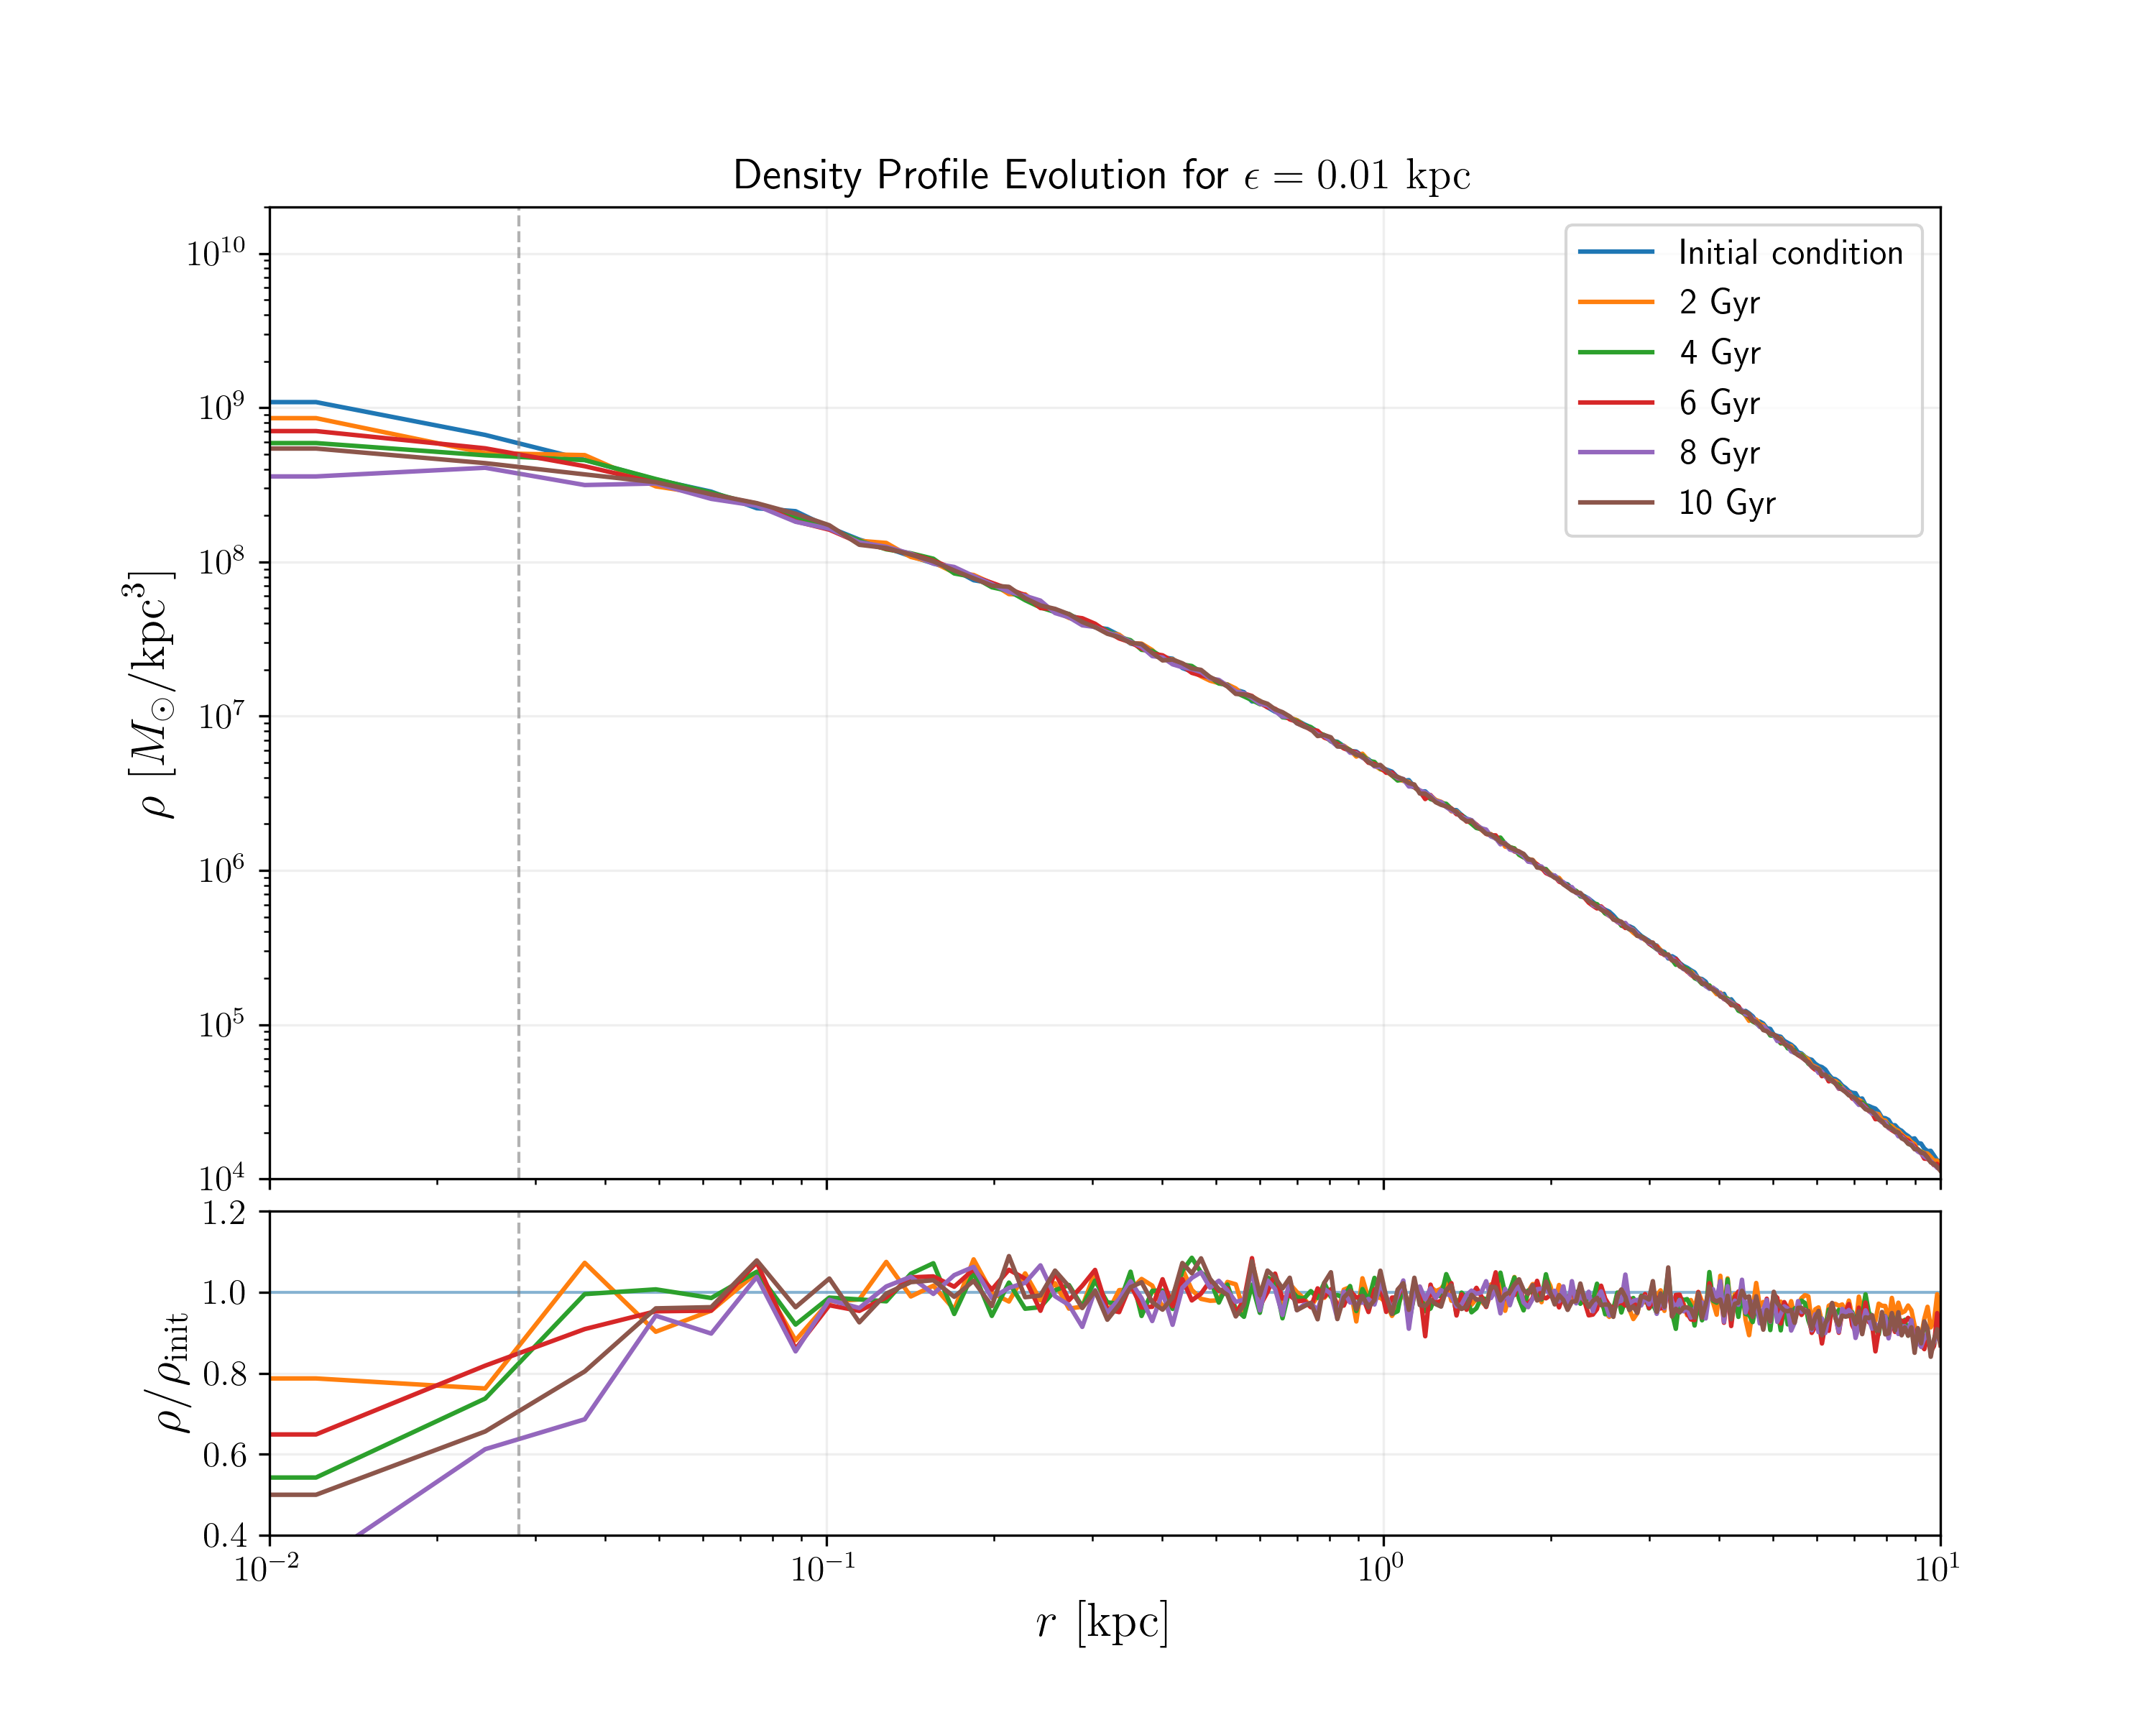
\includegraphics[width=0.48\textwidth]{density_evo_timestep02_10.png}
        \hfill
        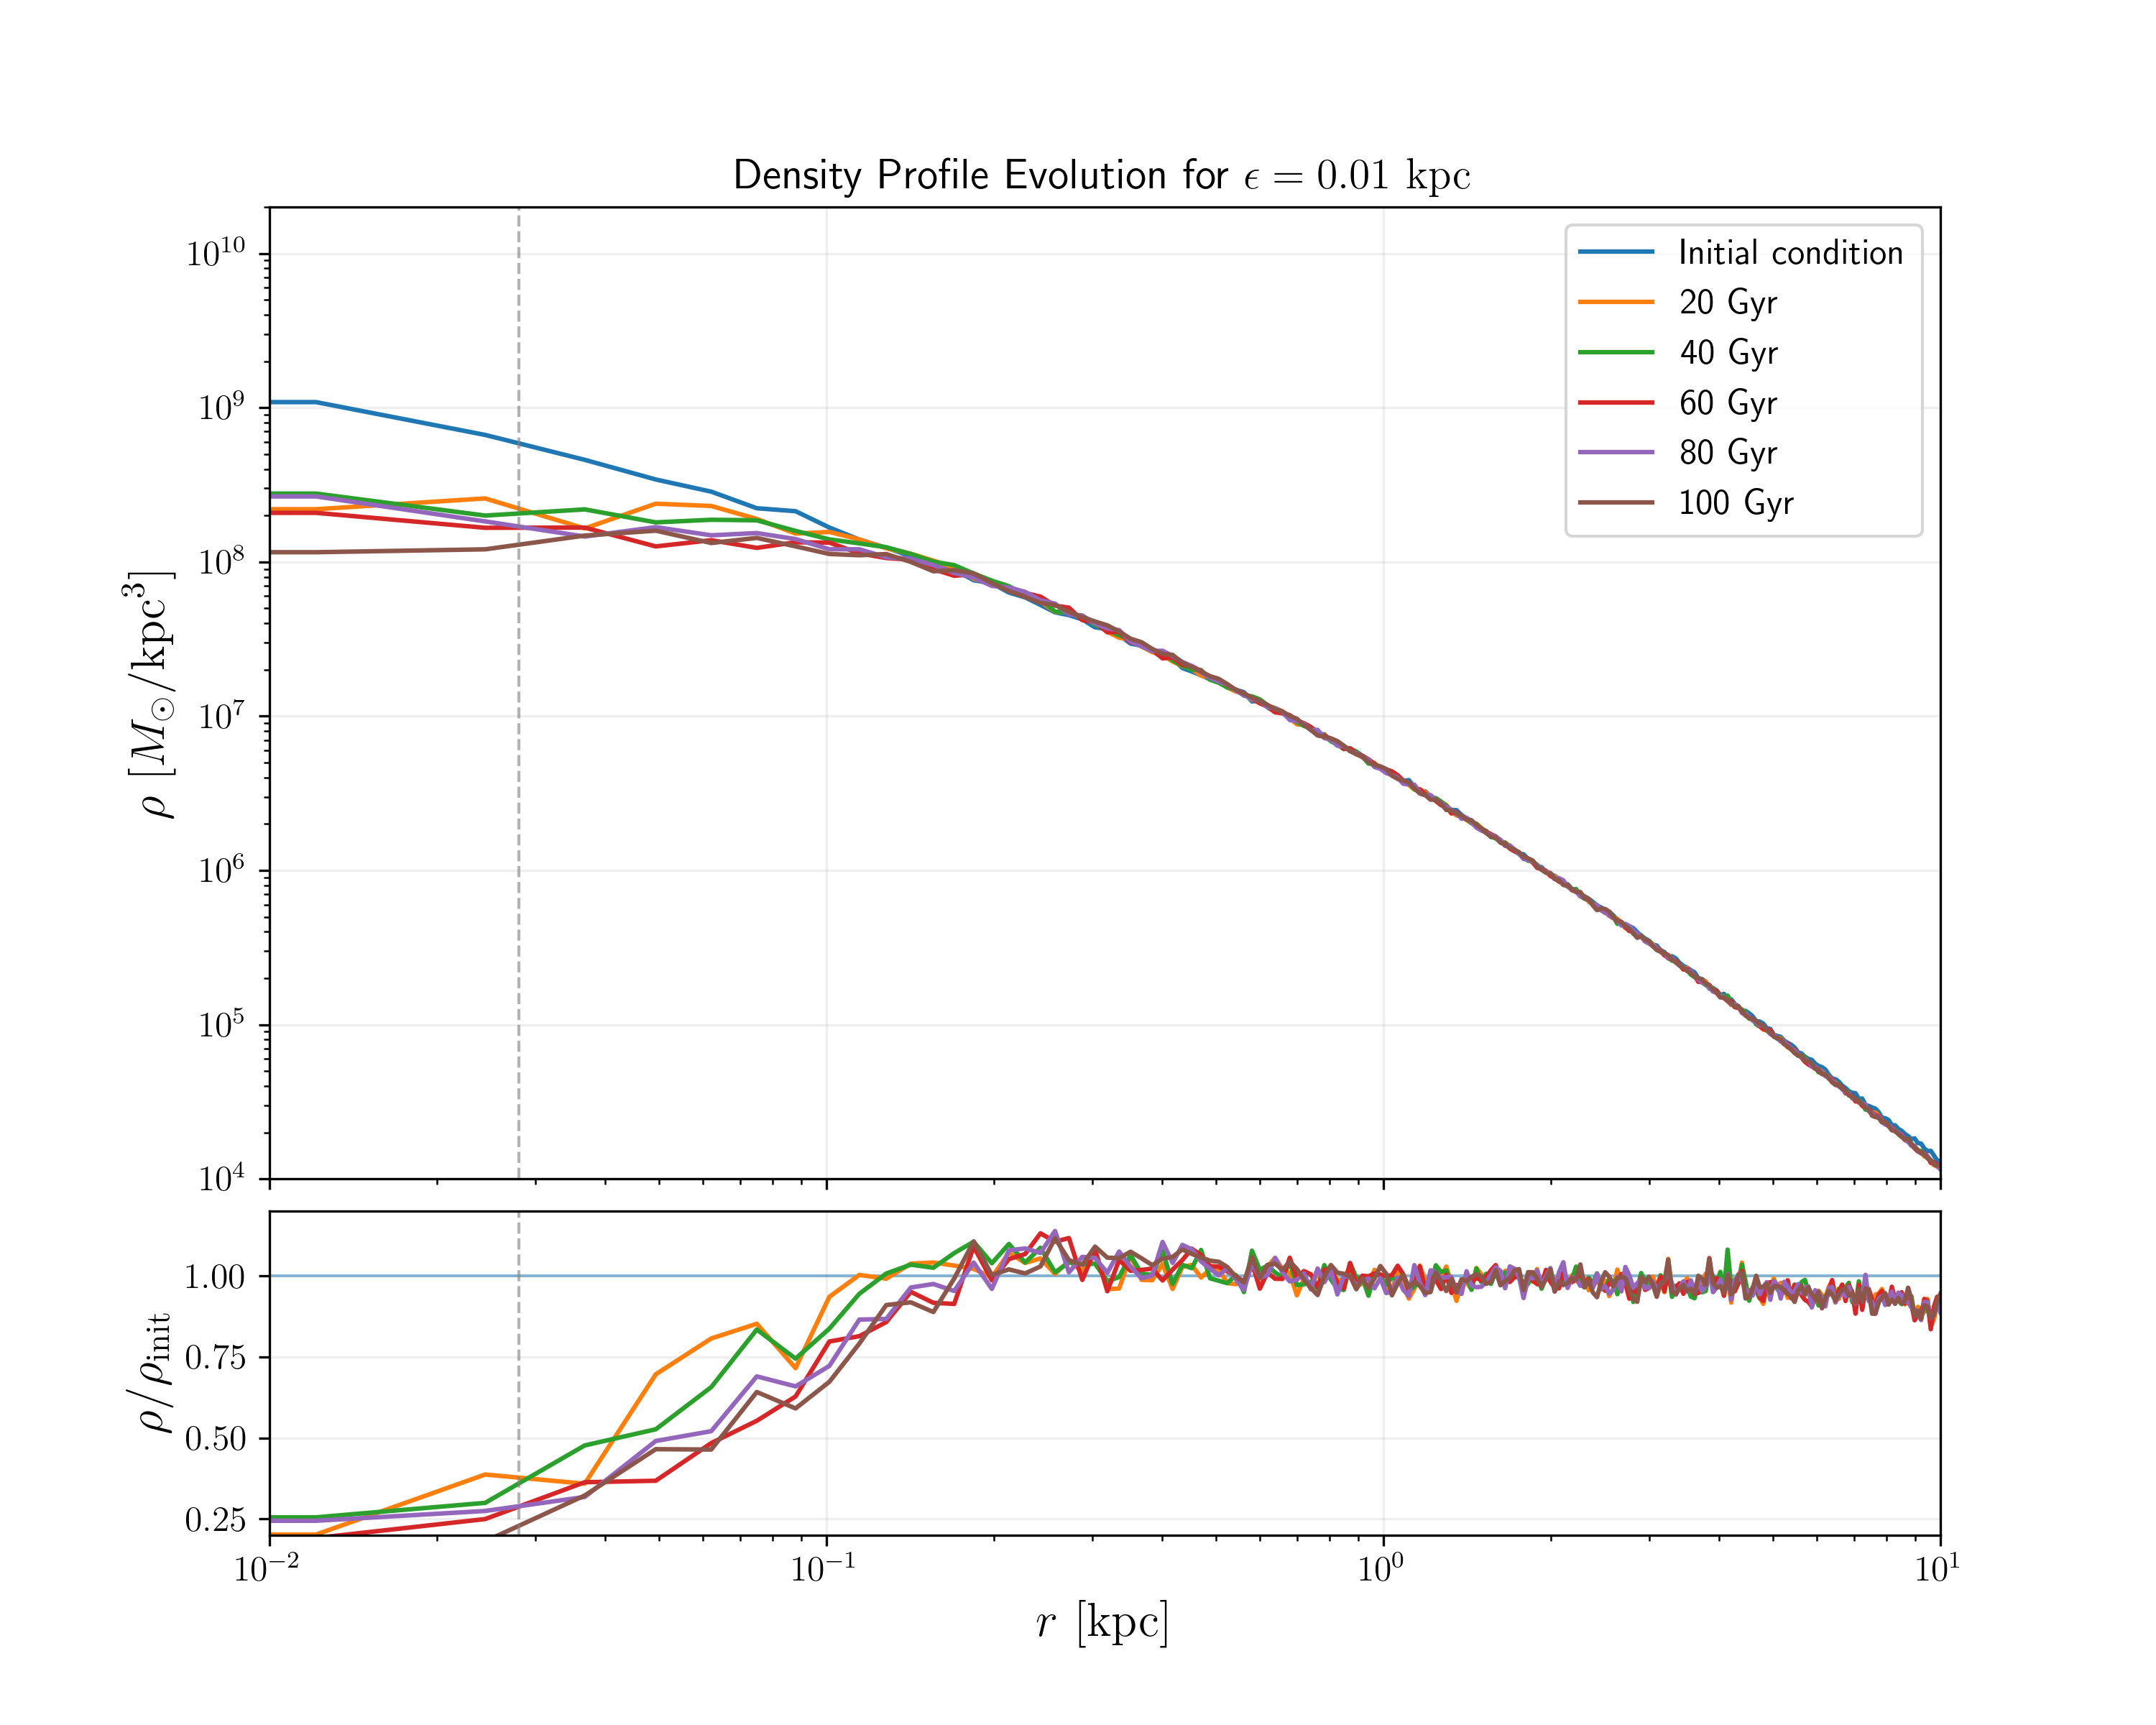
\includegraphics[width=0.48\textwidth]{density_evo_timestep02_100.png}
    \end{minipage}
    \caption{Density evolution for $\eta$ (timestep) tests. Left-to-right, top-to-bottom: $\eta = 0.02$ (step 10), $0.02$ (step 100), $0.0002$ (step 10), $0.0002$ (step 100).}
\end{figure}

\begin{figure}[H]
    \centering
    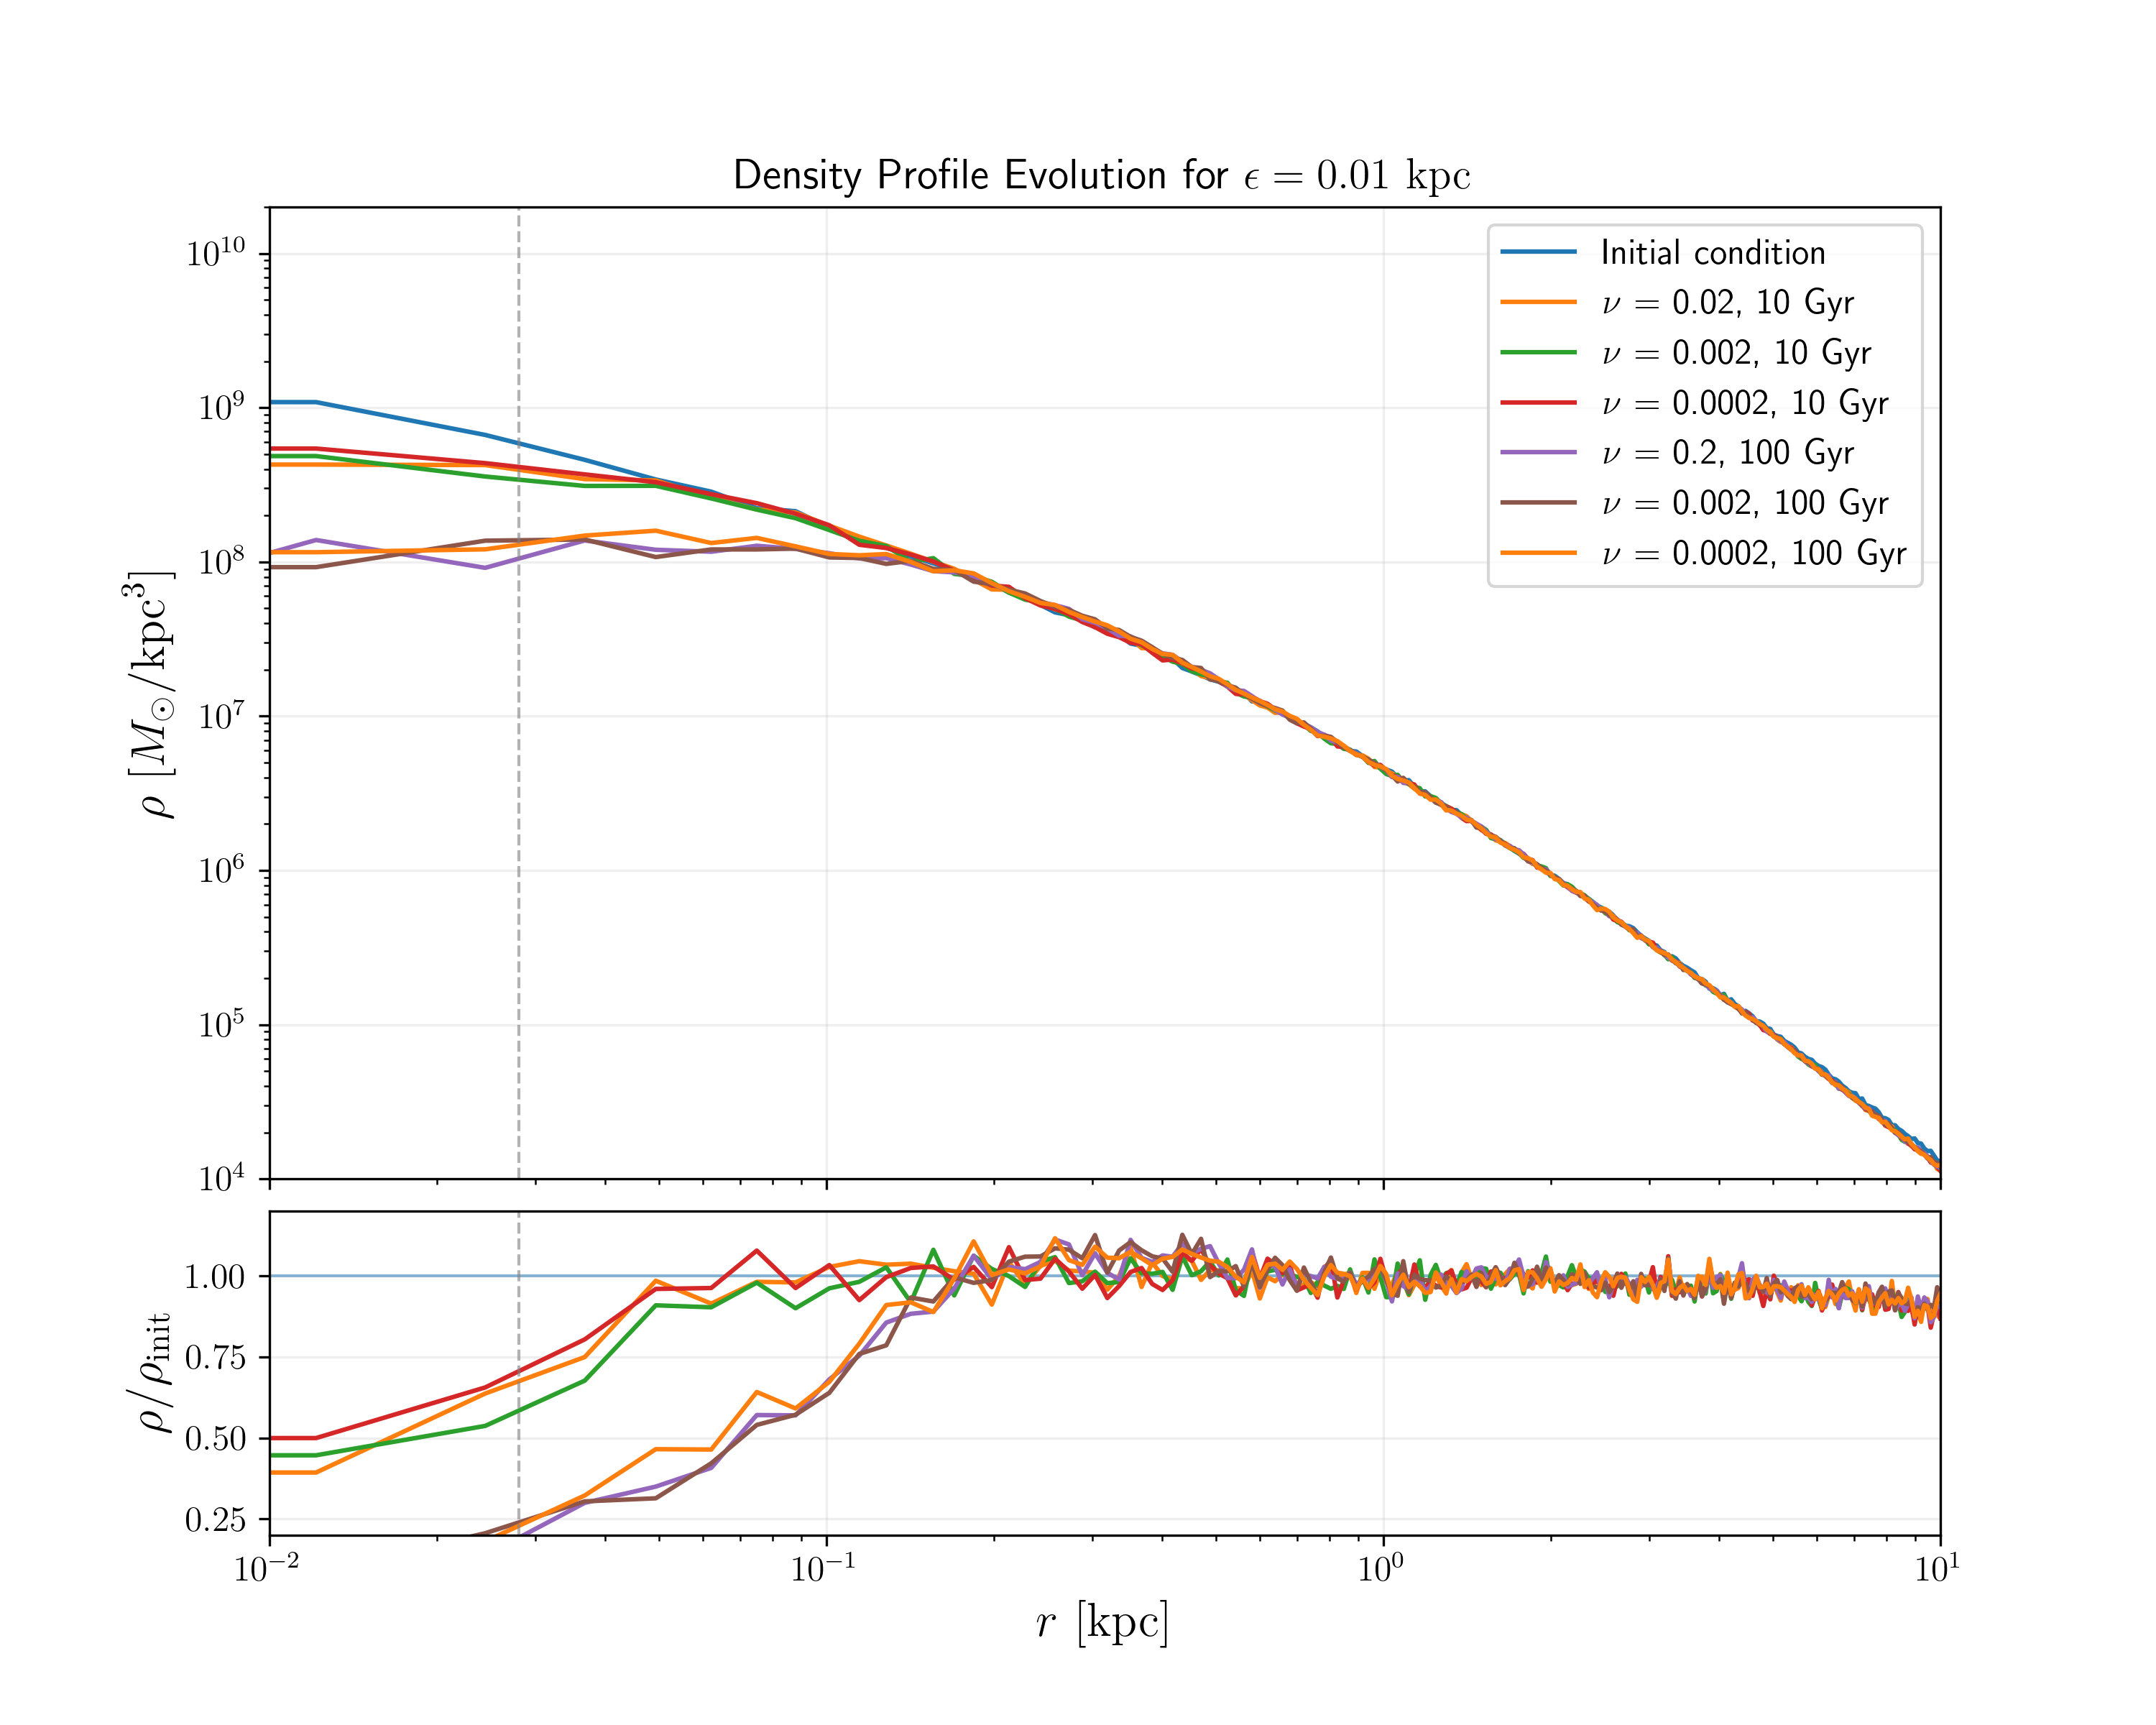
\includegraphics[width=0.95\textwidth]{comp_timestep.png}
    \caption{Comparison of $\eta$ (timestep) sensitivity: baseline 0.002 versus test values 0.0002 and 0.02.}
\end{figure}

\end{document}